\documentclass[a4paper, 12pt]{article}

\usepackage{bookmark}
\usepackage{fontspec}
\usepackage{enumitem}
\usepackage{mathtools}
\usepackage{subcaption}
\usepackage{amsthm,amsmath,amssymb}
\usepackage[ruled, noline]{algorithm2e}
\usepackage[a4paper, rmargin=3cm, lmargin=3cm, top=2.5cm, bottom=2.5cm]{geometry}

\usepackage{listings} % Para formatar o código
\usepackage{tabularx} % Para tabelas ajustáveis à largura total

\lstset{
    basicstyle=\ttfamily\small,
    keywordstyle=\bfseries,
    frame=single,              
    breaklines=true,
    tabsize=4,
    captionpos=b
}

\renewcommand{\lstlistingname}{Objeto}
\renewcommand{\lstlistlistingname}{Lista de Objetos}

\usepackage{setspace}
\setstretch{1.5}
\setlength{\parindent}{1.25cm}
\setlength{\parskip}{6px}

\usepackage{unicode-math}
\setmathfont{Stix Two Math}
\setmathfont{TeX Gyre Pagella Math}[
   range=bb,
   Scale=MatchUppercase,
   version=pagella
]

\usepackage{polyglossia}
\setdefaultlanguage{portuguese} % might be portuguese, though referencing may present incompatibilities
\setotherlanguages{english} % secondary language for abstract and stuff
\usepackage{libertine}

% in case you have a local installation for the font Times, this is preferrable, especially if you have Small Caps support
%\setmainfont{times}[
%  % In my case, needs to point for MS Office location since regular MacOS Times doesn't support small caps
%  Path           = /Applications/Microsoft Word.app/Contents/Resources/DFonts/,
%  Extension      = .ttf ,
%  BoldFont       = *bd ,
%  ItalicFont     = *i ,
%  BoldItalicFont = *bi,
%  Ligatures      = Rare, %for some unknown reason, Times put Common ligatures under Rare
%]

% or simply, in case you have the legal font Times LT Std installed in your local machine
%\setmainfont{Times LT Std}[Ligatures = Common] % name might differ

% useful command defition for writting mathematics: QED, norm, set cardinality and equals by definition
\renewcommand{\qedsymbol}{$\blacksquare$}
\newcommand{\norm}[1]{\left\lVert#1\right\rVert}
\newcommand{\card}[1]{\lvert#1\rvert}
\newcommand*{\defeq}{\mathrel{\vcenter{\baselineskip0.5ex \lineskiplimit0pt
                     \hbox{\scriptsize.}\hbox{\scriptsize.}}}%
                     =}

% useful command definition for SCB bracket citation
\newcommand{\citeb}[1]{\bibleftbracket\cite{#1}\bibrightbracket}

% math numbering scheme, speak with your supervisor in case you want to change it
\newtheorem{theorem}{Theorem}[section]
\newtheorem*{definition}{Definition}
\newtheorem{corollary}{Corollary}[theorem]
\newtheorem{lemma}[theorem]{Lemma}

% reference style (Sociedade Brasileira de Computação is compliant with Chicago author-date)
% as per https://presencial.unifcv.edu.br/arquivos/orientacao_para_artigos_area_informatica.pdf
\usepackage[authordate, strict, backend=biber, autolang=other]{biblatex-chicago}
\addbibresource{references.bib}
\DeclareDelimFormat{nameyeardelim}{\addcomma\space}
\setlength\bibitemsep{6.0pt}

% flush all sections right
\usepackage{sectsty}
\sectionfont{\raggedleft}

% used only for text samples, can be safely removed in the final document
\usepackage{lipsum} 
\usepackage{metalogo}

% used for image rendering
\usepackage{graphicx}
\graphicspath{ {../images/} }

\usepackage{hyperref}
% Personalização dos nomes para \autoref
\renewcommand{\figureautorefname}{Figura} % Substitui "Figure" por "Imagem"
\renewcommand{\tableautorefname}{Tabela} % Substitui "Table" por "Tabela"
\renewcommand{\sectionautorefname}{Seção} % Substitui "Section" por "Seção"
\renewcommand{\subsectionautorefname}{Seção} % Substitui "Subsection" por "Subseção"
\renewcommand{\subsubsectionautorefname}{Seção} % Substitui "Subsubsection" por "Subseção"
\renewcommand{\equationautorefname}{Equação} %

\begin{document}
% Page numbering for early pages and document presentation
\pagenumbering{roman}
\setcounter{page}{1}

\thispagestyle{empty}

    \begin{center}
        \begin{figure}
            \centering
            
\includegraphics[scale=0.18]{unirio.png}
            \label{fig:unirio-logo}
        \end{figure}
        
        \fontsize{13}{15}
        
        \textsc{
            Universidade Federal do Estado do Rio de Janeiro\\
            Centro de Ciências Exatas e Tecnológicas\\
            Escola de Informática Aplicada\\
        }
        \vspace{2.8cm}
        
        \textit{Retrieval Augmented Generation} Aplicado a Bibliotecas\\
        
        \vspace{2.8cm}
        Breno Costa da Silva Filgueiras
        \vspace{2.8cm}

        \begin{flushright}
            \textbf{Orientador}\\
            Pedro Nuno de Souza Moura
        \end{flushright}

        \vspace*{\fill}
        
        \textsc{Rio de Janeiro, RJ -- Brasil\\ Dezembro, 2024}
    \end{center}

    \clearpage

    \begin{center}
        Retrieval Augmented Generation Aplicada à Bibliotecas
        \vskip 0.5cm
        Breno Costa da Silva Filgueiras
        \vskip 2.0cm
    \end{center}

    \begin{flushright}
        \parbox{8.0cm}{
        Projeto de graduação apresentado à Escola de Informática Aplicada
        da Universidade Federal do Estado do Rio de Janeiro (UNIRIO) como
        cumprimento de requerimento parcial para obtenção título de Bacharel em
        Sistemas de Informação.}
        \vskip 1.5cm
        Approved by:
        \vskip 1.5cm
        \rule{10.0cm}{.1mm}

        Pedro Nuno de Souza Moura -- UNIRIO
        \vskip 1.0cm
        
        \rule{10.0cm}{.1mm}

        Carlos Eduardo Mello -- UNIRIO
        \vskip 1.0cm

        \rule{10.0cm}{.1mm}

        Jobson Luiz Massollar da Silva -- UNIRIO
        \vskip 1.0cm
    \end{flushright}
    \vspace{\stretch{1}}
    \begin{center}
        \textsc{Rio de Janeiro, RJ -- Brasil} \\ \textsc{Dezembro, 2024}
    \end{center}
    % Fim da folha de rosto
    \clearpage

    \vfill
    
    \begin{center}
        Catalogação informatizada pelo autor
        % http://www.unirio.br/bibliotecacentral/fichas-catalograficas
    \end{center}

    \clearpage

    \begin{flushright}
        Agradecimentos
    \end{flushright}
    
    Agradeço profundamente aos meus pais, Rita e Alexandre, pelo apoio incondicional ao longo de toda a minha jornada, mas especialmente durante meu percurso acadêmico, sempre ao meu lado.

    Aos meus irmãos, sou grato por me incentivarem a continuar meus estudos e por me lembrarem de que sou um exemplo e uma fonte de inspiração para eles. Estarei sempre com vocês, em cada conquista.
    
    Aos meus amigos, que estiveram ao meu lado durante o processo de escrita, meu sincero agradecimento por me motivarem a seguir em frente, mesmo nos momentos de dificuldade, quando a paciência ou inspiração pareciam escassas.
    
    Um agradecimento especial ao meu orientador, Pedro Nuno de Moura Souza, que me guiou na fascinante jornada pelo universo do \textit{Deep Learning} e Inteligência Artificial. Sua confiança em minhas ideias e o apoio contínuo, especialmente durante a mudança de tema do TCC, foram fundamentais para o sucesso deste trabalho.

    \clearpage

    \begin{abstract}
        Em uma parceria entre Seagate e a International Data Corporation (IDC) foi realizado o estudo \citetitle{digitization}, nele a IDC fala sobre diversos aspectos referentes aos dados presentes no mundo digital e um dos tópicos abordados no estudo é ``Mankind is on a quest to digitize the world'' e neste mesmo tópico eles explicam que os dados que geramos no dia a dia está em constante crescimento, ou seja, estamos gradualmente produzindo mais dados.

        Com um volume cada vez maior de dados, uma busca por informação otimizada é essencial, dado que são necessárias ferramentas que nos garantam confiança e precisão da informação adquirida. Com isso em mente, este trabalho visa o desenvolvimento de um sistema capaz de ler, processar e armazenar documentos diversos de determinada biblioteca (conjunto de documentos) para que possamos utilizar um \textit{Large Language Model} (LLM) para responder perguntas que os usuários possam ter acerca dos documentos.
        
        A ideia é conseguir processar documentos de diferentes épocas, temas, formatos e conseguir responder o maior número possível de perguntas dos usuários com a melhor confiança possível.

        \begin{flushleft}
            \textbf{Palavras-chave:} retrieval, augmented, generation, inteligência, artificial.
        \end{flushleft}
    \end{abstract}
    \clearpage

    \begin{english}
        \begin{abstract}
            In a partnership between Seagate and the International Data Corporation (IDC), the study \citetitle{digitization} was conducted. In it, IDC discusses various aspects related to data present in the digital world and one of the topics covered in the study is ``Mankind is on a quest to digitize the world''. In this same topic, they explain that the data we generate on a daily basis is constantly growing, that is, we are gradually producing more data.

            With an ever-increasing volume of data, an optimized search for information is essential, given that tools are needed that guarantee reliability and accuracy of the information acquired. With this in mind, this work aims to develop a system capable of reading, processing and storing various documents from a given library (set of documents) so that we can use a \textit{Large Language Model} (LLM) to answer questions that users may have about the documents.

            The idea is to be able to process documents from different periods, themes and formats and to be able to answer as many user questions as possible with the greatest possible confidence.

            \begin{flushleft}
                \textbf{Keywords:} retrieval, augmented, generation, artifical, inteligence.
            \end{flushleft}
            
        \end{abstract}    
    \end{english}
    
    \clearpage

    \tableofcontents
    \clearpage

    \listoffigures
    \clearpage

    \listoftables
    \clearpage

    \lstlistoflistings
    \clearpage

    \pagenumbering{arabic}
    \setcounter{page}{1}

    \section{Introdução}

    Com a expansão contínua da Internet das Coisas (IoT), o cenário se transforma em um redemoinho de informações. Chegará, ou talvez já tenha chegado, o momento em que será impossível para qualquer ser humano consumir tudo o que criou em um único dia.

    Durante estudo, a \textit{International Data Coorporation} (IDC) previu que a \textit{Global Datasphere} cresceria de 45 \textit{zettabytes} em 2019 para 175 \textit{zettabytes} em 2025 \citeb{digitization}. Um crescimento de aproximadamente 380\% em 6 anos, porém essa previsão foi feita em 2018 e atualmente já existem estudos que projetam números ainda maiores para a produção de dados. Na \autoref{fig:total_dados_anual}, temos um gráfico gerado durante o estudo \citetitle{data_created}, onde foram calculados um total de 147 \textit{zettabytes} produzidos em 2024, com previsão de 181 \textit{zettabytes} para 2025, um crescimento de 23.12\% \citeb{data_created}.

    \begin{figure}[ht]
        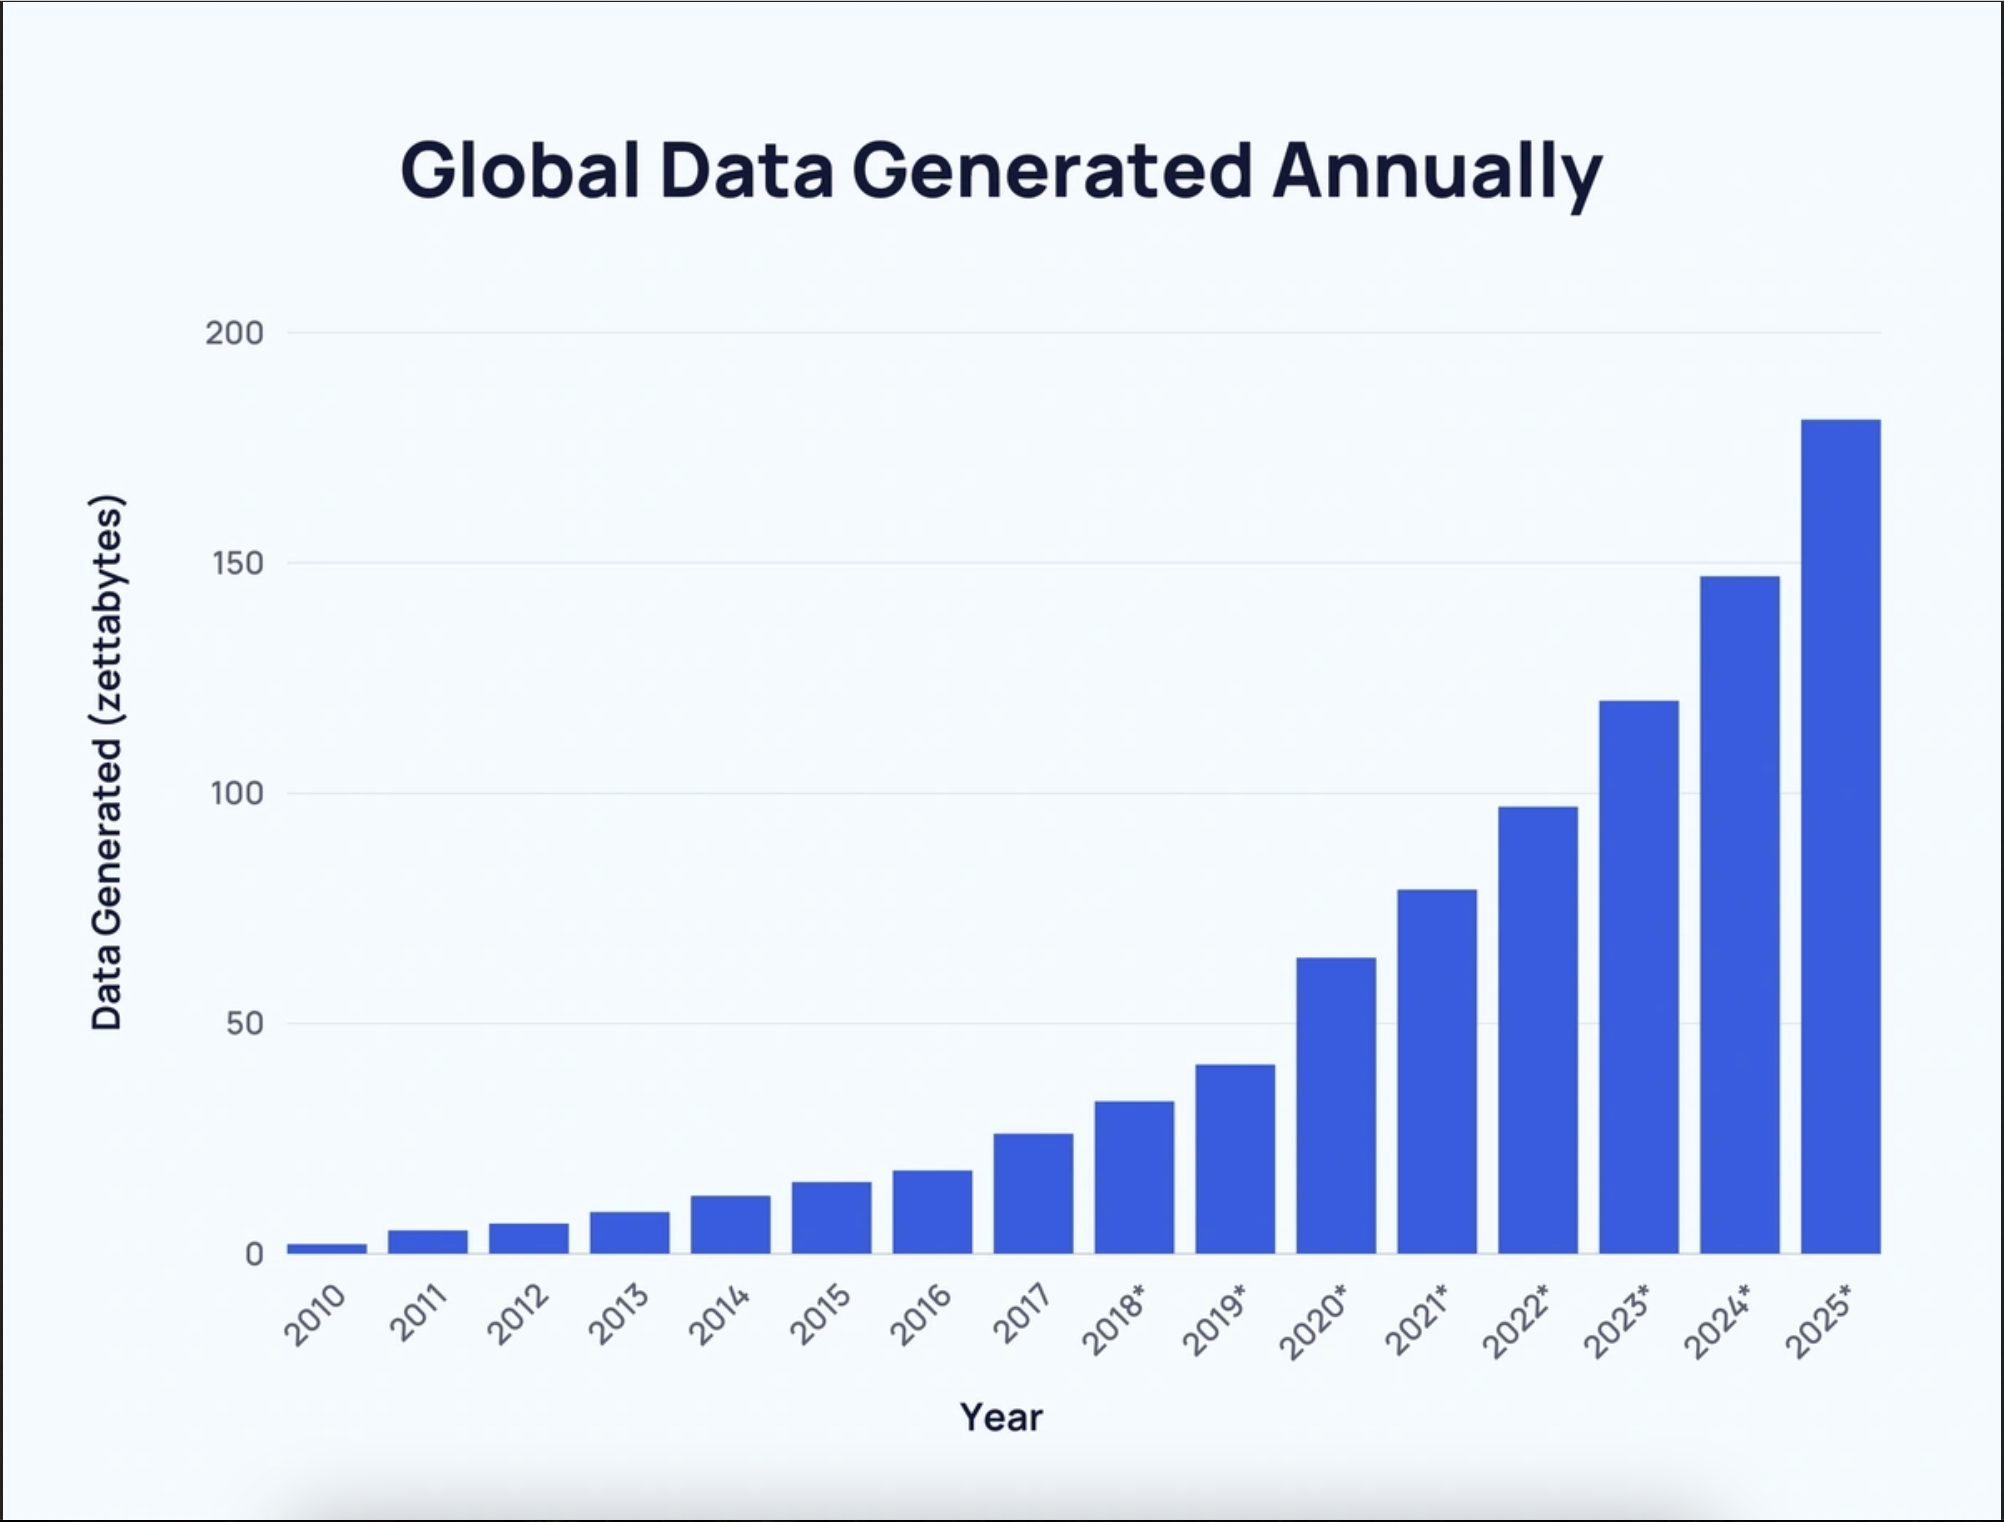
\includegraphics[width=\textwidth,height=0.9\textheight,keepaspectratio]{global-data-generated-annually-fabio-duarte.png}
        \centering
        \caption{Total de dados produzidos por ano (extraído de \citeb{data_created})}
        \centering
        \label{fig:total_dados_anual}
    \end{figure}        

    \subsection{Motivação}

    No estudo \citetitle{digitization}, a \textit{Seagate}, gigante do armazenamento de dados, uniu forças com a \textit{International Data Corporation} (IDC) para conduzir uma análise dos dados presentes na \textit{Global Datasphere}, que quantifica e analisa o total de dados criados, capturados e replicados no mundo inteiro. A IDC destacou: ``\textit{Mankind is on a quest to digitize the world}''. Essa frase encapsula a era em que vivemos, marcada por um crescimento incessante no volume de dados que produzimos diariamente.
    
    Cada clique, pagamento por aproximação ou uso de \textit{wearables} adiciona mais um fragmento ao vasto oceano digital. Nesse turbilhão de dados, buscar uma matéria ou reportagem torna-se uma tarefa semelhante a encontrar uma agulha em um palheiro digital, um desafio tão fascinante quanto frustrante.

    E esse contexto de imensidão de dados onde a busca por informações é cada vez mais dificíl, é o berço deste projeto. O objetivo é implementar uma solução que processe bibliotecas de documentos e aplique o conceito de \textit{Retrieval Augmented Generation} (RAG). Com uma interface de chat simples, o usuário poderá fazer perguntas e receber respostas humanizadas, geradas por um \textit{Large Language Model} (LLM), com referências claras aos documentos de origem.

    O desafio de buscar informações relevantes é significativo. A internet ainda abriga dados sem referência ou apresentados de formas variadas, como gráficos e textos, dificultando a assimilação. Além disso, interfaces pouco intuitivas e mecanismos de busca ineficazes consomem tempo valioso. Para estudantes e pesquisadores, essa batalha constante com a desorganização digital pode transformar o simples ato de encontrar informações em um verdadeiro labirinto.

    \subsection{Objetivos} \label{sec:objectives}

    O objetivo principal deste trabalho é implementar uma solução baseada em \textit{Retrieval Augmented Generation} (RAG) para bibliotecas de documentos específicos, a fim de viabilizar consultas que retornem dados pertinentes junto com suas referências. Os objetivos específicos são:
    
    \begin{enumerate}
        \item Escrever uma introdução acessível ao conceito de RAG aos alunos do Bacharelado em Sistemas de Informação.
        \item Produzir um documento que instrua a implementação de um ecossistema RAG para desenvolvedores ou estudantes.
        \item Realizar a implementação de RAG para documentos, que seja agnóstica tanto ao LLM quanto \textit{embedding} utilizados.
        \item Executar uma validação sobre a solução gerada, de maneira que o resultado seja relevante.
    \end{enumerate}

    \subsection{Organização do Texto}

    Este trabalho está organizado em capítulos, com o objetivo de apresentar os processos, métodos, análises e descobertas de forma clara e coerente. A estrutura do documento foi elaborada para facilitar a compreensão do leitor sobre a complexidade do tema e os resultados obtidos, conduzindo-o até a implementação da solução final. Os capítulos estão estruturados da seguinte forma:
    
    \begin{itemize}
        \item \textbf{Introdução:} Apresenta o contexto do trabalho, destacando o problema do crescente volume de dados. Discute a motivação para a solução proposta, sua relevância no cenário atual e os objetivos estabelecidos.
        \item \textbf{Conceitos Fundamentais:} Dedica-se à fundamentação teórica, abordando os conceitos essenciais para a compreensão da solução e sua implementação. Inclui uma introdução ao conceito de \textit{Large Language Models} (LLM) e uma análise detalhada do \textit{Retrieval Augmented Generation} (RAG).
        \item \textbf{Modelagem:} Descreve a composição da solução, explicando os componentes envolvidos e suas responsabilidades. Também aborda o funcionamento e o papel de cada componente na solução final. Ao final, apresenta as tecnologias utilizadas, incluindo descrições breves sobre as ferramentas, suas versões e funções.
        \item \textbf{Solução Desenvolvida:} Detalha os componentes implementados, explicando como a solução cumpre suas funções. Apresenta os resultados obtidos e discute as respostas fornecidas para algumas das questões propostas, avaliando a eficácia da solução.
        \item \textbf{Conclusão:} O capítulo final resume as considerações sobre os resultados alcançados, destacando tanto os aspectos positivos quanto as limitações da solução implementada. Além disso, discute possíveis trabalhos futuros ou aplicações derivadas da solução, encerrando com as referências utilizadas no desenvolvimento do trabalho.
    \end{itemize}

    \subsection{Metodologia}

    Este trabalho adotará a abordagem de \textit{Design Science Research} (DSR) para garantir que, ao final do trabalho, o artefato modelado esteja implementado e funcionando conforme planejado, atendendo aos requisitos definidos e demonstrando sua viabilidade prática. O DSR oferece uma estrutura robusta para guiar a criação de soluções baseadas em evidências, alinhando teoria e prática de forma estruturada.

    Com raízes na engenharia e nas ciências do artificial \citeb{simon_1996}, o DSR é uma metodologia voltada para a resolução de problemas. Seu objetivo é aprimorar o conhecimento humano por meio da criação de artefatos inovadores e da geração de conhecimento de design, oferecendo soluções práticas para problemas do mundo real \citeb{design_science}. 
    
    No artigo \citetitle{dsr} \citeb{dsr}, é apresentado um diagrama que detalha o processo de pesquisa do DSR, a tradução deste diagrama apresentada na \autoref{fig:dsr_model} expõe quatro pontos de entrada para o início do processo de pesquisa:
    
    \begin{enumerate}
        \item Iniciação centrada no problema
        \item Solução centrada no objetivo
        \item Iniciação centrada no desenho e no desenvolvimento
        \item Iniciado por cliente ou contexto
    \end{enumerate}
    
    Neste trabalho, o início do processo de pesquisa é feito através da iniciação centrada no problema, discutido na \autoref{sec:problem}. A aplicação do DSR valoriza a integração de análise teórica com resultados práticos, incentivando a reflexão crítica sobre as escolhas metodológicas e de \textit{design} realizadas durante o projeto.
    
    \begin{figure}[ht]
        \includegraphics[width=\textwidth,height=0.9\textheight,keepaspectratio]{dsrm-process-model-2.png}
        \centering
        \caption{Tradução do diagrama do processo de pesquisa do DSR (extraído de \citeb{dsr})}
        \centering
        \label{fig:dsr_model}
    \end{figure}  

    Isso possibilita uma contribuição mais ampla, tanto para o avanço acadêmico quanto para a aplicação prática em contextos organizacionais. Assim, ao utilizar o DSR, este trabalho resultará em um artefato produzido com base nas análises e discussões realizadas ao longo das próximas seções deste trabalho.
    
    \clearpage

    \section{Conceitos Fundamentais} \label{sec:concepts}

    Para que este trabalho seja compreendido e os próximos capítulos possam ser apresentados com maior clareza, é necessário passar por alguns conceitos. Antes de nos aprofundarmos no contexto de um ecossistema de \textit{retrieval augmented generation} (RAG), é necessário compreender um pouco a IA generativa e os \textit{Large Language Models} (LLMs) que contribuem tanto para a interpretação das perguntas feitas durante as interações com o usuário quanto na geração de uma resposta mais humana.

    \subsection{IA Generativa}
    
    A inteligência artificial generativa (IA generativa), às vezes chamada de \textit{gen AI} (\textit{Generative AI}), é um tipo de inteligência artificial (IA) capaz de criar conteúdo original — como texto, imagens, vídeos, áudio ou código de \textit{software} — em resposta a um comando ou solicitação do usuário. \citeb{genai_ibm}

    A IA generativa baseia-se em modelos avançados de \textit{machine learning} (aprendizado de máquina) chamados de modelos de \textit{deep learning} (aprendizagem profunda) — algoritmos que se inspiram na estrutura do cérebro humano e o seu processo de aprendizado. Esses modelos trabalham identificando padrões e relações em grandes volumes de dados.

    A partir de um treinamento em uma base de dados de tamanho massivo (da ordem de trilhões de palavras), a IA generativa é capaz de compreender solicitações ou perguntas feitas em linguagem natural pelos usuários, respondendo com conteúdos novos e relevantes. Essa capacidade permite a criação de textos, imagens, vídeos, áudios e até códigos de software, de forma original e adaptada ao pedido do usuário.


    \subsubsection{Uma Breve História}

    O termo ``IA generativa'' explodiu na consciência pública na década de 2020, mas a inteligência artificial já faz parte de nossas vidas há décadas, e a tecnologia de IA generativa atual tem seus pilares contruídos desde o século XX. Uma história representativa não exaustiva da IA generativa pode incluir algumas das seguintes datas:

    \begin{itemize}
        \item \textbf{1964:} O cientista da computação do \textit{Massachusetts Institute of Technology} (MIT), Joseph Weizenbaum, desenvolve o ELIZA, uma aplicação de processamento de linguagem natural baseada em texto. Essencialmente o primeiro \textit{chatbot} (chamado de ``\textit{chatterbot}'' na época), o ELIZA usava \textit{scripts} de correspondência de padrões para responder a entradas de linguagem natural digitadas com respostas empáticas em texto.

        \item \textbf{1999:} A Nvidia lança a GeForce, a primeira unidade de processamento gráfico (\textit{Graphic Processing Unit} - GPU). Originalmente desenvolvida para fornecer gráficos de movimento suave para videogames, as GPUs se tornaram a plataforma padrão para o treinamento de modelos de IA e mineração de criptomoedas, por conta de sua alta capacidade de cálculo matricial.

        \item \textbf{2004:} O Google \textit{autocomplete} aparece pela primeira vez, gerando palavras ou frases potenciais à medida que os usuários digitam seus termos de busca.

        \item \textbf{2013:} Aparecem os primeiros \textit{autoencoders} variacionais (VAEs).

        \item \textbf{2014:} Surgem as primeiras redes adversariais generativas (GANs) e modelos de difusão.

        \item \textbf{2017:} Ashish Vaswani, junto com uma equipe do Google Brain e um grupo da Universidade de Toronto publicam o artigo \textit{Attention is All you Need}, \citeb{att_all_u_need}, um artigo que documenta os princípios dos modelos de \textit{transformers}, amplamente reconhecidos como os responsáveis por permitir os modelos de fundação mais poderosos e as ferramentas de IA generativa que estão sendo desenvolvidas e utilizadas atualmente.

        \item \textbf{2019-2020:} A OpenAI lança seus modelos de linguagem GPT (\textit{Generative Pre-trained Transformer}), o GPT-2 e o GPT-3.
    
        \item \textbf{2022:} O OpenAI apresenta o ChatGPT, uma interface de \textit{chatbot} do GPT-3 que gera frases complexas, coerentes e contextuais, além de conteúdo de longo formato em resposta a comandos dos usuários.
        
        \item \textbf{2023-2024:} Com a notoriedade e popularidade do ChatGPT, que efetivamente abriu as portas para uma onda de desenvolvimentos, os avanços e lançamentos de produtos em IA generativa têm ocorrido a um ritmo acelerado, incluindo lançamentos do Google Bard (agora Gemini), Microsoft Copilot, IBM watsonx.ai e o modelo de linguagem Llama-2 de código aberto da Meta.
    \end{itemize}

    A inteligência artificial tem sido um tema relevante na tecnologia, mas foi a IA generativa, especialmente com o lançamento do ChatGPT em novembro de 2022, que a destacou globalmente, gerando inovação e adoção. Ela oferece grandes benefícios de produtividade para indivíduos e organizações, e, apesar dos desafios e riscos, as empresas exploram como melhorar fluxos de trabalho e enriquecer produtos e serviços. De acordo com uma pesquisa da consultoria \textit{McKinsey}, mais de 65\% das empresas usam Gen AI no mundo. \citeb{mckinsey_genai}.


    \subsection{Large Language Models}

    Os \textit{Large Language Models} (LLMs) são uma categoria de modelos fundamentais treinados em grandes volumes de dados para oferecer capacidades versáteis, atendendo a diversos casos de uso e tarefas. Diferentemente dos modelos específicos para determinados domínios, que exigem treinamentos separados para cada aplicação—geralmente com altos custos e demandas significativas de infraestrutura—os LLMs promovem uma aplicação mais ampla, gerando sinergias entre diferentes áreas e, muitas vezes, alcançando um desempenho superior. \citeb{llm_ibm}

    Os LLMs representam um avanço significativo em \textit{Natural Language Processing} (NLP) e inteligência artificial. Esses modelos estão amplamente acessíveis ao público por meio de LLMs como o \textit{ChatGPT-3} e \textit{GPT-4} da \textit{OpenAI}, apoiados pela \textit{Microsoft}. Outros exemplos incluem os modelos \textit{Llama} da Meta, os modelos \textit{BERT/RoBERTa} e \textit{PaLM} do Google, e a série \textit{Granite} lançada pela IBM.

    Os LLMs são projetados para compreender e gerar texto de forma similar à humana, além de produzir outros tipos de conteúdo. Com base nos extensos volumes de dados em que foram treinados, conseguem traduzir idiomas, resumir textos, responder perguntas, auxiliar na redação e até mesmo na geração de código.

    Essas capacidades são viabilizadas por bilhões de parâmetros que capturam padrões complexos da linguagem. Como resultado, os LLMs estão transformando áreas como \textit{chatbots}, assistentes virtuais, geração de conteúdo, suporte à pesquisa e tradução de idiomas.

    \subsubsection{Como funcionam?}

    Os \textit{Large Language Models} (LLMs) operam utilizando técnicas de aprendizagem profunda e grandes volumes de dados textuais. Baseados na arquitetura de \textit{transformers} \citeb{att_all_u_need}, como o \textit{Generative Pre-trained Transformer} (GPT), esses modelos são especialmente eficazes em lidar com dados sequenciais, como entradas de texto. Compostos por várias camadas de redes neurais, os LLMs empregam um mecanismo de atenção para focar em partes específicas da sequência de texto fornecida na entrada.

    Durante o treinamento, os modelos aprendem a prever um conjunto de próximas palavras em uma sentença com base no contexto fornecido pelas palavras anteriores e posteriores. Isso é feito atribuindo probabilidades à recorrência de palavras que foram transformadas em \textit{tokens} (divididas em sequências menores) e geradas as \textit{embeddings}, representações numéricas que capturam o contexto de ocorrência das palavras.

    O treinamento envolve o uso de \textit{corpora} (conjuntos de textos) massivos, com bilhões de páginas de texto e trilhões de palavras, permitindo que os LLMs aprendam gramática, semântica e relações conceituais por meio de aprendizado auto-supervisionado, modelagem de sequência e demais técnicas de treinamento de LLMs. Uma vez treinados, os modelos geram texto prevendo autonomamente as próximas palavras com base na entrada recebida e nos padrões aprendidos, resultando em uma produção linguística coerente e relevante para diversas tarefas de compreensão e geração de linguagem.

    O desempenho dos LLMs pode ser aprimorado por meio de técnicas como \textit{prompt engineering}, \textit{fine-tuning} (ajuste fino) e aprendizado por reforço com feedback humano (\textit{Reinforcement Learning from Human Feedback} - RLHF). Essas abordagens ajudam a mitigar problemas como viés, discurso de ódio e respostas incorretas ou ilusórias (\textit{hallucinations}). Garantir que os LLMs estejam prontos para uso, seja em sociedade ou nível corporativo, é crucial para evitar riscos à reputação e responsabilidades indesejadas.
    
    \subsection{Padrões de Projeto} \label{sec:design_pattern}

    Os padrões de projeto (\textit{Design Patterns}) são soluções reutilizáveis para problemas recorrentes no desenvolvimento de software. Eles foram formalizados no clássico livro \citeb{design_patterns} e são amplamente utilizados para melhorar a estrutura, a legibilidade e a manutenção de sistemas. Suas principais vantagens incluem:
    
    \begin{itemize}
        \item \textbf{Abstração}: Simplificam a complexidade ao ocultar os detalhes de implementação;
        \item \textbf{Reutilização de Código}: Reduzem redundâncias, promovendo um desenvolvimento mais eficiente;
        \item \textbf{Flexibilidade}: Facilitam a adaptação de sistemas a novos requisitos sem modificar significativamente o código existente;
        \item \textbf{Manutenção e Escalabilidade}: Tornam o sistema mais modular e fácil de ajustar ao longo do tempo.
    \end{itemize}
    
    \subsubsection{Padrão de Fábrica} \label{sec:factory_pattern}

    Neste trabalho, o padrão fábrica será utilizado em situações em que a abstração de um serviço ou classe traz uma vantagem para o componente, de modo que ele possa instanciar uma classe a partir de determinado contexto, como é ilustrado na \autoref{fig:factory-pattern}.
    
    \begin{figure}[ht]
        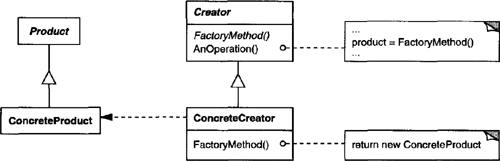
\includegraphics[width=\textwidth,height=0.9\textheight,keepaspectratio]{images/factory-design-pattern.jpg}
        \centering
        \caption{Estrutura do \textit{factory design pattern} (extraída de \citeb{design_patterns}).}
        \centering
        \label{fig:factory-pattern}
    \end{figure}
    
    O padrão de fábrica, é um padrão criacional que fornece uma interface para a criação de objetos em uma superclasse, delegando às subclasses a responsabilidade de determinar qual classe concreta será instanciada. Ele é útil quando a criação de objetos envolve lógica complexa ou quando diferentes tipos de objetos precisam ser criados de forma dinâmica, dependendo do contexto. Como ilustrado na \autoref{fig:factory-pattern}, o padrão de fábrica implementa uma interface para a criação de objetos que herdam de uma superclasse, permitindo que as classes filhas possam alterar o tipo de objeto criado. 

    
    \subsection{O Problema} \label{sec:problem}

    No livro \citetitle{rothman}, é dito que ``mesmo o modelo mais avançado de Inteligência Artificial (IA) generativa é limitado a responder somente sobre dados nos quais ele foi treinado.'' \citeb{rothman}. Essa afirmação chama a atenção para um problema especial: como fazer para que uma IA saiba responder perguntas referentes a um conjunto específico de dados, diferente daquele em que foi treinada?

    Quando um modelo de IA generativo não sabe como responder com precisão, alguns dizem que ele está produzindo viés ou sofrendo uma \textit{hallucination} (alucinação). No entanto, ``tudo se resume à impossibilidade de fornecer uma resposta adequada quando o treinamento do modelo não incluiu as informações solicitadas, além dos problemas clássicos de configuração do modelo.'' \citeb{rothman}. Essa confusão geralmente leva a sequências aleatórias das saídas mais prováveis, não das mais precisas.

    Buscando mitigar essas questões, em 2020 foi publicado o artigo \citetitle{RAG} \citeb{RAG}, que combinava abordagens baseadas em recuperação com modelos generativos, introduzindo o \textit{Retrieval Augmented Generation} (RAG). Um RAG recupera dados relevantes de fontes externas em tempo real e usa esses dados para gerar respostas contextualmente relevantes, isto é, que façam sentido dentro do contexto trabalhado durante as consultas feitas pelo usuário. Uma de suas principais vantagens é a adaptabilidade, tendo em vista que a estrutura pode ser aplicada independentemente do tipo de dado abordado na solução, seja texto, imagens, áudios ou documentos diversos.


    \subsection{Retrieval Augmented Generation (RAG)}
    
    Quando um modelo de IA generativa não sabe responder determinada pergunta com precisão, diz-se que ele está alucinando ou apresentando viés, mas, na prática, está apenas gerando respostas sem sentido. Isso ocorre porque o modelo não foi treinado com as informações solicitadas ou por conta de limitações em sua configuração, resultando em sequências prováveis, mas não precisas, necessariamente.

    Um RAG começa onde a IA generativa termina, fornecendo informações que um modelo de LLM não possui para responder com precisão às consultas do usuário. Um RAG otimiza tarefas de recuperação de informações e adiciona os dados recuperados durante a entrada (seja consulta do usuário ou um \textit{prompt} automatizado), gerando uma saída melhorada e mais amigável ao usuário. O funcionamento geral do RAG pode ser resumido na \autoref{fig:rag_estudante}, que será explicada nos próximos parágrafos:

    \begin{figure}[h]
        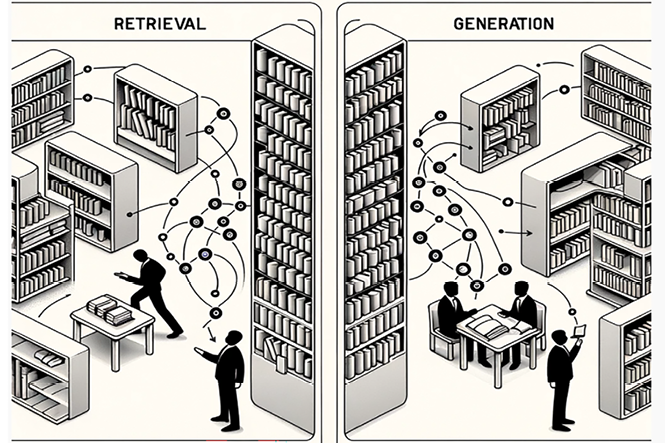
\includegraphics[width=\textwidth,height=0.9\textheight,keepaspectratio]{retrieval-generation-denis-rothman.png}
        \centering
        \caption{Funcionamento geral de uma estrutura RAG (extraída de \citeb{rothman})}
        \centering
        \label{fig:rag_estudante}
    \end{figure}

    Imagine um estudante em uma biblioteca, com a tarefa de escrever uma dissertação sobre RAG. Assim como o ChatGPT ou outras ferramentas de IA generativa, o estudante sabe ler e escrever. Como qualquer LLM, o estudante é treinado para compreender informações avançadas, resumir e criar conteúdo. No entanto, como qualquer IA, há muitas informações que este estudante ainda desconhece.

    Na fase de recuperação, ele busca por livros sobre o tema necessário (lado esquerdo da \autoref{fig:rag_estudante}) na biblioteca. Em seguida, ele retorna ao seu lugar, realiza a tarefa de recuperação sozinho ou com a ajuda de um colega, extraindo as informações relevantes dos livros adquiridos. Na fase de geração (lado direito da \autoref{fig:rag_estudante}), o estudante começa a escrever a sua dissertação utilizando o conhecimento adquirido na fase anterior. Esse é o funcionamento de um agente humano guiado por RAG, de maneira semelhante a uma estrutura de IA generativa baseada em RAG.

    Enquanto escreve sua dissertação sobre RAG, o estudante encontra tópicos difíceis com os quais não tem tempo para consultar todas as informações disponíveis. Como um agente humano generativo, ele fica travado, assim como um modelo de IA generativa. Ele até pode tentar escrever algo sobre esses tópicos, mas, como a IA, não saberá se o conteúdo está correto até que alguém corrija a dissertação e lhe avalie de alguma maneira.

    Neste ponto, ele já atingiu seu limite e decide recorrer a uma ferramenta de IA generativa com RAG para obter respostas corretas e auxiliá-lo. No entanto, existe uma grande variedade de modelos de LLM e configurações RAG disponíveis, deixando o estudante sobrecarregado. Antes de prosseguir, é necessário entender os recursos disponíveis e como o RAG está organizado.

    \subsection{Ecossistema RAG}

    A IA generativa baseada em RAG é um \textit{framework} que pode ser implementada com diversas configurações, funcionando dentro de um ecossistema amplo (\autoref{fig:rag_framework}). Independentemente da quantidade de estruturas de recuperação e geração disponíveis, tudo se resume a quatro eixos principais e suas respectivas questões:
    
    \begin{itemize}
        \item \textbf{Dados:} De onde vêm os dados? São confiáveis e suficientes? Há questões de direitos autorais, privacidade ou segurança?
        \item \textbf{Armazenamento:} Como os dados serão armazenados antes ou depois do processamento? Qual será o volume armazenado?
        \item \textbf{Recuperação:} Como os dados corretos serão recuperados para complementar a entrada (ou consulta) do usuário? Qual tipo de \textit{framework} RAG será mais adequado ao projeto?
        \item \textbf{Geração:} Qual modelo de IA generativa melhor se adapta ao \textit{framework} RAG escolhido?
    \end{itemize} 

    Esses eixos dependem do tipo de \textit{framework} RAG utilizado. Antes de escolher, é essencial avaliar a proporção de conhecimento paramétrico e não paramétrico no ecossistema implementado. No contexto de aprendizado de máquina, o conhecimento paramétrico é o entendimento internalizado que um modelo ganha com o treinamento em um conjunto de dados. 
    
    Esse conhecimento é representado pelos parâmetros do modelo (pesos e viéses), que são ajustados durante o processo de treinamento para minimizar a função de perda e melhorar o desempenho do modelo. O conhecimento paramétrico permite que o modelo faça previsões e generalize para dados novos e invisíveis, capturando recursos e relacionamentos essenciais dentro dos dados de treinamento.

    \clearpage

    \begin{figure}[ht]
        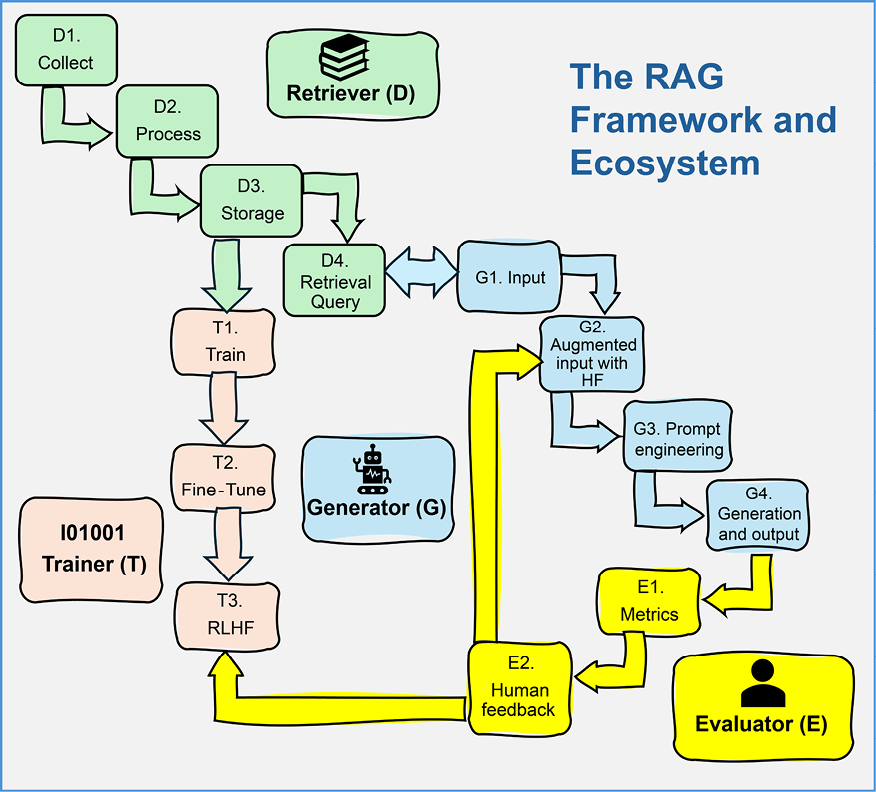
\includegraphics[width=\textwidth,height=0.9\textheight,keepaspectratio]{rag-framework-ecosystem-denis-rothman.png}
        \centering
        \caption{Arquitetura da estrutura RAG (extraída de \citeb{rothman})}
        \centering
        \label{fig:rag_framework}
    \end{figure}

    Como ilustrado acima, na \autoref{fig:rag_framework}, são ilustrados quatro componentes que dependem de seus respectivos ecossistemas, compostos por seus subcomponentes, formando o \textit{pipeline} de IA generativa baseada em RAG. Estes componentes são: 
    
    \begin{itemize}
        \item \textbf{\textit{Retriever}} (D, em verde na \autoref{fig:rag_framework}): Responsável pela coleta, processamento, armazenamento e recuperação de dados.
        \item \textbf{\textit{Generator}} (G, em azul na \autoref{fig:rag_framework}): Cuida da complementação da entrada, engenharia de prompts e geração de respostas.
        \item \textbf{\textit{Evaluator}} (E, em amarelo na \autoref{fig:rag_framework}): Avalia o desempenho usando métricas matemáticas, \textit{feedback} humano e outras formas de validação.
        \item \textbf{\textit{Trainer}} (T, em rosa na \autoref{fig:rag_framework}): Gerencia o modelo pré-treinado inicial e sua posterior ajuste fino (\textit{fine-tuning}).
    \end{itemize}

    Nas seções seguintes, serão usadas as siglas D, G, E e T para representar,respectivamente, \textit{Retriever}, \textit{Generator}, \textit{Evaluator} e \textit{Trainer}.

    \subsubsection{\textit{Retriever} (D)}

    O componente \textit{retriever} de um ecossistema RAG coleta, processa, armazena e recupera dados. O ponto de partida de um ecossistema RAG é, portanto, um processo de ingestão de dados, cujo primeiro passo é a coleta de dados. Os subcomponentes são:

    \begin{enumerate}
        \item \textbf{Coleta de Dados (D1):} Atualmente dados são extremamente diversos, podendo ser textos, arquivos de mídia (como músicas ou vídeos em mp4) ou arquivos estruturados e não estruturados (PDFs, JSONs e páginas \textit{web}). Além disso, grande parte desses dados é não estruturada e pode ser encontrada de maneiras imprevisíveis e complexas. Felizmente, várias plataformas, como Pinecone \footnote{\citeurl{pinecone}}, OpenAI \footnote{\citeurl{openai}}, Chroma \footnote{\citeurl{chroma}} e Activeloop \footnote{\citeurl{activeloop}}, oferecem ferramentas prontas para processar e armazenar essa vasta quantidade de dados.
        \item \textbf{Processamento de Dados (D2):} Na fase de coleta de dados (D1) no processamento de dados multimodais, diferentes tipos de dados, como texto, imagens e vídeos, podem ser extraídos de \textit{websites} utilizando técnicas de \textit{web scraping} ou outras fontes de informação. Esses objetos de dados são então transformados para criar representações uniformes. Alguns exemplos dessas transformações incluem: \textit{chunking}, \textit{embedding} e indexação. Essas técnicas serão discutidas mais adiante.
        \item \textbf{Armazenamento de Dados (D3):} Neste estágio do \textit{pipeline}, já se coletou e se iniciou o processamento de uma grande quantidade de dados diversos. Mas para fazermos com que esses dados sejam úteis, deve-se fazer uso de \textit{vector stores} (armazenamento de vetores), como Elastic Search. Esse não apenas armazena os dados, mas os convertem em entidades matemáticas, representadas como vetores, permitindo realizar cálculos poderosos. Esses sistemas também utilizam técnicas de indexação e outras abordagens para garantir acesso rápido e eficiente aos dados. Em vez de manter os dados em arquivos estáticos, transforma-se tudo em um sistema dinâmico e pesquisável, pronto para alimentar \textit{chatbots}, motores de busca e outras aplicações.
        \item \textbf{Consulta de Recuperação (D4):} \label{sec:recovery} O processo de recuperação é acionado pela entrada (ou consulta) do usuário ou entrada automatizada (G1). Para recuperar dados rapidamente, carregamos os dados nos \textit{vector stores} e \textit{datasets} após transformá-los para um formato adequado. Em seguida, utilizamos uma combinação de pesquisas por palavras-chave, \textit{embeddings} inteligentes e indexação para recuperar os dados de forma eficiente.
        A equação da similaridade cosseno, definida na \autoref{eq:cosseno}, como: 
        
        \begin{equation}
            \text{sim}_{\cos}(\vec{x}, \vec{y}) = \frac{\vec{x} \cdot \vec{y}}{\|\vec{x}\|_2 \|\vec{y}\|_2}
            \label{eq:cosseno}
        \end{equation}
        
        Calcula o cosseno entre dois vetores, por exemplo, encontra itens (vetores) que estejam intimamente relacionados, garantindo que os resultados da busca não sejam apenas rápidos, mas também altamente relevantes.
    \end{enumerate}

    Após a recuperação dos dados, o próximo passo é aumentar a entrada, ou seja, adicionar as informações recuperadas para enriquecer a resposta gerada ao usuário.

    \subsubsection{\textit{Generator} (G)}

    No ecossistema RAG, as linhas entre a entrada e a recuperação não são tão nítidas, como mostrado na \autoref{fig:rag_framework}, que representa o \textit{framework} e ecossistema RAG. A entrada do usuário (G1), seja automatizada ou humana, interage com a consulta de recuperação (D4) para complementar a entrada antes de enviá-la ao modelo generativo. O fluxo gerativo começa com a entrada do usuário, que é aprimorada com dados recuperados antes de ser processada pelo modelo de IA generativa.

    \begin{enumerate}
        \item \textbf{Entrada (G1):} A entrada pode ser uma série de tarefas automatizadas (como o processamento de \textit{e-mails}, por exemplo) ou \textit{prompts} humanos por meio de uma Interface de Usuário (\textit{User Interface} - UI). Essa flexibilidade permite integrar a IA de forma flúida em diversos ambientes profissionais, aprimorando a produtividade em diferentes setores.
        \item \textbf{Entrada Aumentada com Feedback Humano (G2):} O feedback humano (\textit{Human Feedback} - HF) pode ser adicionado à entrada, conforme descrito na \autoref{sec:human_feedback}, sob o componente \textit{evaluator} (E). O \textit{feedback} humano torna o ecossistema RAG consideravelmente mais adaptável, permitindo total controle sobre a recuperação de dados e as entradas para a IA generativa.
        \item \textbf{Engenharia de \textit{Prompts} (G3):} Tanto o \textit{retriever} (D) quanto o \textit{generator} (G) dependem fortemente da engenharia de \textit{prompts} para preparar a mensagem padrão e aumentada que o modelo de IA generativa deverá processar. A engenharia de \textit{prompts} combina a saída do \textit{retriever} (D) com a entrada do usuário, garantindo que o modelo receba uma entrada bem estruturada e relevante para gerar a resposta desejada.
        \item \textbf{Geração e Saída (G4):} A escolha de um modelo de IA generativa (LLM) depende dos objetivos do projeto. Modelos como Llama \footnote{\citeurl{llama_models}}, Gemini\footnote{\citeurl{gemini_models}}, GPT \footnote{\citeurl{gpt_models}} e outros podem atender a diferentes requisitos. No entanto, o \textit{prompt} precisa estar alinhado com as especificações de cada modelo.
    \end{enumerate}

    \subsubsection{\textit{Evaluator} (E)}

    Frequentemente, dependemos de métricas matemáticas para avaliar o desempenho de um modelo de IA generativa (LLM). No entanto, essas métricas fornecem apenas uma parte do todo. É importante lembrar que o teste final da eficácia de uma IA depende da avaliação humana, que garante uma compreensão mais completa da qualidade e aderência aos objetivos do usuário.

    \begin{enumerate}
        \item \textbf{Métricas (E1):} Um modelo não pode ser avaliado sem métricas matemáticas, como a similaridade cosseno, assim como em qualquer sistema de IA. Essas métricas garantem que os dados recuperados sejam relevantes e precisos. Ao quantificar as relações e a relevância dos \textit{data points}, elas fornecem uma base sólida e objetiva para avaliar o desempenho e a confiabilidade do modelo. Fidelidade, ou seja, se a resposta está fundamentada no contexto recuperado. Relevância da resposta, ou seja, se a resposta atende à pergunta e relevância do contexto, se o contexto recuperado é suficientemente focado.
        \item \textbf{Feedback Humano (E2):} \label{sec:human_feedback} Em um sistema de IA generativa, seja ele baseado em RAG ou não, independentemente de as métricas matemáticas parecerem suficientes, o \textit{feedback} humano é essencial. A avaliação humana é o fator decisivo que determina se um sistema projetado para usuários humanos será aceito ou rejeitado, elogiado ou criticado.
    \end{enumerate}
    
    \subsubsection{\textit{Trainer} (T)}

    Um modelo de IA generativa padrão é pré-treinado em uma grande quantidade de dados de propósito geral. Em seguida, podemos ajustar finamente (\textit{fine-tuning}, T2) o modelo com dados específicos de um determinado domínio.
    
    \clearpage
    
    \section{Modelagem}

    Com os conceitos de um ecossistema RAG em mente, é possível explicar de forma objetiva a modelagem da solução proposta para este trabalho. Antes de abordar as tecnologias específicas, tema reservado para um capítulo posterior, será apresentada uma visão abstrata da modelagem da solução.

    A solução foi modelada com base no padrão arquitetural para aplicações RAG proposto por \citeauthor{ibm_rag} no texto \textit{\citetitle{ibm_rag}} \citeb{ibm_rag}, onde são apresentados modelos conceituais de uma arquitetura específica para soluções que façam uso do RAG.

    De maneira objetiva, o projeto pode ser descrito como um sistema composto por três componentes, cada um responsável por uma parte do ecossistema proposto. Esses componentes implementam sistemas ou serviços que se comunicam entre si ao longo da solução, podendo implementar uma LLM, uma API ou uma instância de banco vetorial. Apesar de estarem conectados, cada componente é independente e funciona de forma autônoma.
    
    Juntos, esses três componentes formam a solução proposta. Proporcionando uma abordagem modular e integrada para alcançar os objetivos propostos neste trabalho, que resultará em um ecossistema explicado mais à frente, na \autoref{sec:ecosystem}. Dentre os componentes que serão explicados a seguir, existem, respectivamente, um pipeline de ingestão, um orquestrador (API) e uma interface gráfica de usuário.
    
    \subsubsection{\textit{Pipeline} de Ingestão} \label{sec:pipeline}

    Para este trabalho, é possível definir um \textit{pipeline} como uma sequência estruturada e organizada de etapas ou processos interconectados, projetada para transformar entradas em saídas de maneira sistemática e eficiente. Cada etapa do \textit{pipeline} irá desempenhar uma função específica, recebendo os dados ou insumos de uma fase anterior, processando-os e, em seguida, encaminhando os resultados para a próxima etapa. Esse fluxo contínuo permite automatizar tarefas complexas, reduzir falhas e otimizar o uso de recursos. 
    
    A ideia central de um \textit{pipeline} é promover eficiência e continuidade ao integrar processos de forma harmoniosa, garantindo que cada componente contribua para o objetivo final com precisão e agilidade. Essa abordagem é amplamente aplicada em diversas áreas, como computação, engenharia de software e operações industriais, destacando sua versatilidade e importância para melhorar fluxos de trabalho e resultados. 

    O \textit{pipeline} de ingestão implementado é responsável por gerenciar fluxos de análise e transformação de documentos para a solução. Neste contexto, ele desempenha a função de lidar com bibliotecas de documentos, analisando cada documento e garantindo que cada um seja processado corretamente, como ilustrado na \autoref{fig:pipeline_scheme}. Esse conjunto de processos compõe o pipeline de ingestão:
    
    \begin{figure}[ht]
        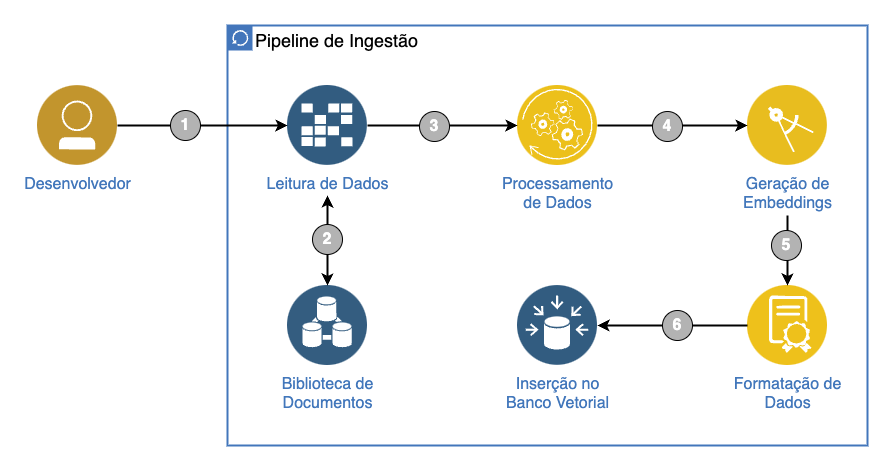
\includegraphics[width=\textwidth,height=0.9\textheight,keepaspectratio]{architecture-pipeline.png}
        \centering
        \caption{Visão arquitetural do \textit{pipeline} de ingestão proposto no trabalho.}
        \centering
        \label{fig:pipeline_scheme}
    \end{figure}
    
    O \textit{pipeline} em questão executa as seguintes etapas: 
    
    \begin{enumerate}
        \item \textbf{Configuração de Ambiente}: o desenvolvedor responsável por executar o \textit{pipeline} configura um arquivo de ambiente contendo as informações referentes ao modelo de \textit{embedding}, LLM utilizado, entre outros.
        \item \textbf{Busca e Leitura de Dados}: um \textit{script} é responsável por buscar os documentos da biblioteca de documentos configurada. Em seguida, a biblioteca é analisada, seus documentos são processados e transformados de maneira sequencial para obtermos objeto específico com as informações necessárias de cada documento.
        \item \textbf{Processamento de Dados}: uma vez extraídos, os dados obtidos são analisados e somente dados relevantes para a operação são guardados em um objeto específico.
        \item \textbf{Geração de \textit{Embeddings}}: para cada objeto obtido na etapa anterior, a informação de cada \textit{chunk} (uma parte do conteúdo do documento particionado) precisa estar em um formato específico para o banco vetorial, este formato é obtido quando geramos os \textit{embeddings}, que neste contexto, são uma representação numérica (vetorial) de baixa dimensão dos dados de um \textit{chunk} específico.
        \item \textbf{Formatação de Dados}: com os \textit{embeddings} da etapa anterior, o objeto com as informações desejadas é completo e se encontra pronto para a inserção no banco vetorial.
        \item \textbf{Inserção no Banco Vetorial}: uma vez gerados, os \textit{embeddings} de cada \textit{chunk} estão presentes no objeto previamente adquirido na etapa de \textbf{Processamento de Dados}. O armazenamento é feito de forma sequencial em \textit{batches}, grupos com tamanho limitado pelo desenvolvedor, através do orquestrador (\textit{Application Programming Interface} - API) já que ela é o único componente com acesso direto ao banco vetorial. Assim, o tempo da etapa de inserção ao banco é reduzido, tendo em vista que, uma vez que um documento é particionado em \textit{chunks}, dependendo do seu tamanho original, podemos obter mais de 100 \textit{chunks}, ou seja, 100 inserções.
    \end{enumerate}
    
    \subsubsection{Orquestrador (API)} \label{sec:api_concept}

    Uma interface de programação de aplicações (\textit{Application Programming Interface} - API), de acordo com \citeauthor{ibm_api}, é um conjunto de regras ou protocolos que permite que aplicativos de software se comuniquem entre si para trocar dados, recursos e funcionalidades \citeb{ibm_api}. Elas são utilizadas para simplificar processos complexos, expondo apenas as funcionalidades necessárias e ocultando detalhes internos, proporcionando uma interface padronizada para o desenvolvedor.

    No contexto da comunicação entre sistemas, uma API geralmente opera através de requisições HTTP, em que um cliente envia uma solicitação a um servidor que, por sua vez, responde com os dados ou serviços solicitados. As APIs podem utilizar formatos como JSON ou XML para a troca de informações. Elas desempenham um papel crucial na construção de aplicações modernas, pois permitem que diferentes softwares interajam sem a necessidade de entender a implementação interna do outro.

    As APIs permitem o compartilhamento apenas das informações necessárias, mantendo outros detalhes internos do sistema ocultos, o que ajuda na segurança do sistema. Servidores ou dispositivos não precisam expor dados completamente — as APIs permitem o compartilhamento de pequenos pacotes de dados, relevantes para a solicitação específica \citeb{ibm_api}. Elas são amplamente utilizadas para fornecer funcionalidades específicas, como acesso a bancos de dados, integração com redes sociais, pagamento eletrônico, entre outros. E também são fundamentais no desenvolvimento de microsserviços e sistemas distribuídos, permitindo que diferentes componentes de uma aplicação se comuniquem de forma eficiente e escalável. 
    
    Dessa forma, a API se torna o componente central no ecossistema proposto, sendo responsável por mediar a comunicação entre os diferentes componentes implementados. Sua principal função é receber e processar as requisições feitas pelos usuários na interface gráfica do usuário (\textit{Graphical User Interface} - GUI), garantindo que as operações sejam realizadas de forma eficiente e segura. Desempenhando um papel crítico na segurança do sistema ao restringir o acesso direto ao banco vetorial por parte dos outros componentes. Essa camada de abstração impede interações não autorizadas ou inadequadas com o banco de dados, garantindo que apenas as operações de usuários autenticados sejam realizadas. 
    
    Com isso, a API promove uma integração controlada e otimizada entre os componentes, além de assegurar a integridade dos dados e a consistência do sistema como um todo.
    
    \subsubsection{Interface Gráfica de Usuário (GUI)} \label{sec:gui}
    
    A interface gráfica do usuário (\textit{Graphical User Interface} - GUI) é um componente essencial no design de sistemas, oferecendo elementos visuais, como botões, menus e janelas, que tornam a interação com o sistema mais intuitiva e acessível. Sua principal função é facilitar o uso das funcionalidades disponíveis, garantindo uma experiência simplificada para o usuário.

    Além de atuar como ponto de interação direta, a GUI funciona como intermediária entre o usuário e a API do sistema. Ela interpreta ações, como cliques ou comandos, e as traduz em requisições para o \textit{backend}, assegurando o processamento correto das instruções.
    
    Com isso, a GUI cumpre um papel estratégico ao integrar a complexidade técnica do sistema com a necessidade de uma interface prática e funcional, promovendo uma comunicação eficiente entre o usuário e a lógica interna do sistema.

    O fluxo de comunicação, ilustrado na \autoref{fig:gui_scheme}, possibilita que tarefas como busca e enriquecimento de respostas ocorram de maneira transparente e alinhadas às necessidades do usuário.

    \clearpage

    \begin{figure}[h!]
        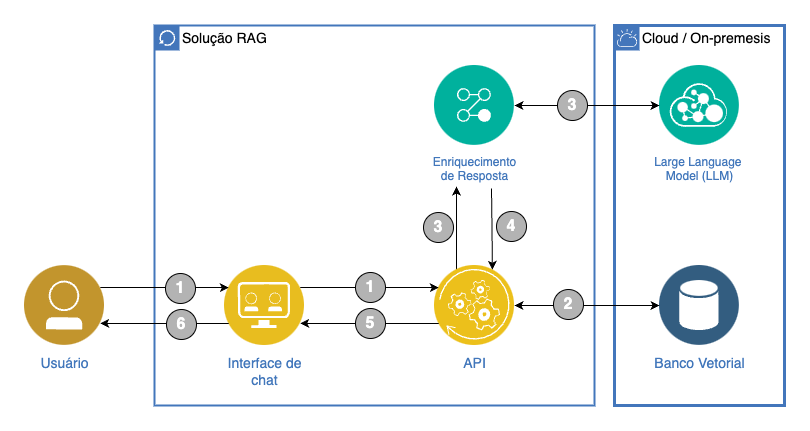
\includegraphics[width=\textwidth,height=0.9\textheight,keepaspectratio]{architecture-solution.png}
        \centering
        \caption{Visão arquitetural do fluxo da interface de usuário proposta no trabalho.}
        \centering
        \label{fig:gui_scheme}
    \end{figure}
    
    A interação do usuário com a interface de \textit{chat}, ilustrado na \autoref{fig:gui_scheme}, pode ser decomposto em seis etapas:
    
    \begin{enumerate}
        \item \textbf{Envio de Consultas (\textit{Query})}: usuário realiza uma pergunta para o \textit{chat}. Em seguida, a interface envia a consulta do usuário para o orquestrador e aguarda a resposta.
        \item \textbf{Busca por Contexto}: No momento em que o usuário realiza a \textit{query}, o sistema realiza uma busca por contexto ou informações relevantes, gerando um objeto de contexto que contém todas as informações relevantes.
        \item \textbf{Enriquecimento da Resposta}: com o contexto da \textit{query}, o orquestrador responde com uma lista contendo os objetos presentes no banco vetorial cujo \textit{embedding} contém informações relevantes para a consulta do usuário.
        \item \textbf{Resposta Enriquecida}: a partir da resposta obtida anteriormente, a lista é encaminhada para um LLM que irá analisar primeiramente um \textit{prompt} focado em entregar respostas humanizadas para o usuário. Nesse \textit{prompt}, o desenvolvedor tem liberdade para criar regras e contextos aos quais o serviço de LLM irá interpretar. Garantindo que o desenvolvedor possa realizar as afinações necessárias para seu próprio contexto.
        \item \textbf{Recebimento da Resposta}: a interface gráfica recebe a resposta da requisição feita ao orquestrador e a expõe para o usuário dentro do modelo de \textit{chat} proposto.
        \item \textbf{Visualização}: o usuário visualiza a resposta humanizada gerada para sua consulta.
    \end{enumerate}

    Essa mediação entre usuário e sistema não apenas melhora a experiência de uso, mas também assegura que a interface seja sincronizada com os demais componentes do sistema. Ao integrar as funcionalidades visuais com a lógica subjacente do sistema, a GUI contribui para uma experiência de interação consistente, eficiente e intuitiva, promovendo um equilíbrio ideal entre acessibilidade e desempenho técnico.
    
    \subsection{Ecossistema RAG} \label{sec:ecosystem}
    
    Analisar uma biblioteca de documentos pode ser complexo, pois cada biblioteca pode comportar diversos tipos de documentos, em formatos distintos. Este projeto foi construído visando à análise de qualquer biblioteca de documentos, ou seja, o processamento dos dados da biblioteca será realizado mesmo que ela tenha arquivos em formatos diferentes. A \autoref{fig:ecosystem} demonstra uma visão geral do ecossistema, que foi implementado com base nos três componentes previamente explicados:

    \begin{figure}[ht]
        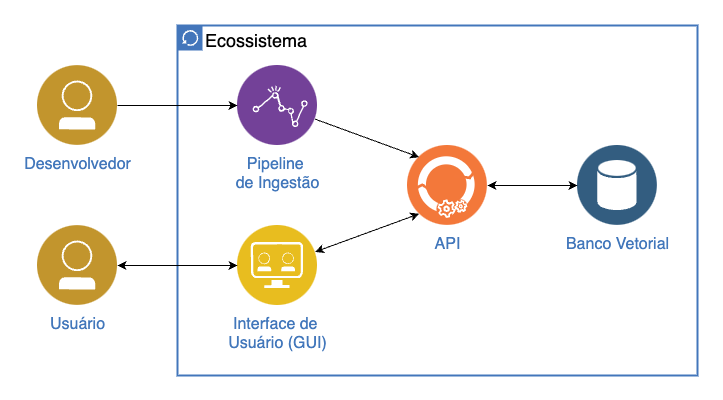
\includegraphics[width=\textwidth,height=0.9\textheight,keepaspectratio]{ecosystem.png}
        \centering
        \caption{Visão arquitetural do ecossistema RAG proposto no trabalho.}
        \centering
        \label{fig:ecosystem}
    \end{figure}

    \subsection{Tecnologias} \label{sec:technologies}

    Este capítulo apresenta as tecnologias utilizadas no desenvolvimento do projeto, destacando suas funcionalidades e relevância para atender aos objetivos propostos. Serão abordadas as ferramentas empregadas na criação da interface, orquestrador, no gerenciamento de dados (banco vetorial) e nas integrações, evidenciando como cada uma contribuiu para a construção de uma solução eficiente e alinhada às melhores práticas.

    \subsubsection{Python e Ambientes Virtuais} \label{sec:python}
    
    O Python 3.11 \footnote{\citeurl{python}} é uma das versões da linguagem de programação Python, lançada com melhorias significativas em desempenho, novas funcionalidades e correções de \textit{bugs}. Uma das principais inovações dessa versão é a otimização do tempo de execução, com um aumento significativo na velocidade em relação às versões anteriores, devido a melhorias no interpretador e na execução de código. 
    
    Além disso, a versão 3.11 introduziu aprimoramentos na sintaxe, como a simplificação de anotações de tipos e novos recursos que facilitam o desenvolvimento de aplicativos mais robustos e eficientes. A linguagem continua a ser uma das mais populares, especialmente em áreas como desenvolvimento \textit{web}, ciência de dados e inteligência artificial.
    
    Ambientes virtuais são espaços isolados em que é possível instalar e gerenciar dependências específicas de um projeto, sem afetar o sistema global ou outros projetos. Em Python, esses ambientes são criados com o módulo venv, permitindo que cada projeto tenha suas próprias versões de pacotes e bibliotecas. Isso evita conflitos entre dependências e facilita o gerenciamento de diferentes versões de pacotes para cada projeto.

    Ambientes virtuais possuem a capacidade de isolar dependências, garantindo que cada projeto utilize a versão correta de pacotes, a facilidade de replicar e compartilhar ambientes de desenvolvimento e a redução de problemas de compatibilidade entre pacotes ou versões do Python. Eles oferecem um controle mais preciso sobre o ambiente de execução, tornando o desenvolvimento mais seguro e eficiente.

    \subsubsection{Docling} \label{sec:docling}

    O Docling \footnote{\citeurl{docling}} é uma biblioteca Python projetada para facilitar a extração e organização de documentos. Ela permite que desenvolvedores processem automaticamente documentos de diferentes formatos, como \textit{PDFs}, textos e arquivos \textit{Word}, para extrair informações estruturadas e relevantes. A biblioteca é útil para automatizar tarefas de leitura e processamento de grandes volumes de dados, organizando-os de forma a facilitar a análise posterior.

    A principal vantagem do Docling é a sua capacidade de simplificar o processo de extração de dados, tornando-o mais rápido e eficiente, sem a necessidade de escrever código complexo para lidar com diferentes tipos de documentos. Isso a torna uma ferramenta valiosa para projetos que requerem análise de texto ou a criação de bancos de dados a partir de documentos não estruturados.

    \subsubsection{Llama Index} \label{sec:llama_index}

    O LlamaIndex \footnote{\citeurl{llama_index}} é uma biblioteca Python que serve como uma estrutura flexível para integrar modelos de LLMs a dados privados, facilitando a construção de assistentes de conhecimento personalizados.

    A biblioteca oferece ferramentas para iniciantes e usuários avançados. Sua API de alto nível permite que iniciantes façam tanto a ingestão quanto a consulta de seus dados com poucas linhas de código, enquanto as APIs de baixo nível possibilitam que usuários avançados personalizem e estendam módulos conforme suas necessidades. O LlamaIndex possui mais de 300 pacotes de integração disponíveis, permitindo que os desenvolvedores escolham os provedores de LLM, \textit{embeddings} e armazenamentos vetoriais que melhor atendam às suas necessidades.

    Em resumo, o LlamaIndex é uma ferramenta poderosa para desenvolvedores que desejam construir assistentes de conhecimento baseados em LLMs, oferecendo flexibilidade e uma ampla gama de integrações para se adaptar a diversos casos de uso.

    \subsubsection{Elastic Search} \label{sec:elasticsearch}

    O Elasticsearch \footnote{\citeurl{elasticsearch}} é um mecanismo de busca e análise distribuído, de código aberto, desenvolvido em Java e baseado no Apache Lucene. Lançado inicialmente em 2010, ele permite armazenar, buscar e analisar grandes volumes de dados em tempo quase real, oferecendo respostas em milissegundos.

    Uma das principais vantagens do Elasticsearch é sua capacidade de lidar com diversos tipos de buscas — estruturadas, não estruturadas, geoespaciais e métricas — permitindo combinar diferentes tipos de consultas de forma eficiente. Além disso, sua natureza distribuída possibilita o processamento paralelo de grandes volumes de dados, garantindo alto desempenho e escalabilidade. Ele é amplamente utilizado em diversos casos de uso, incluindo busca de texto completo, monitoramento de \textit{logs}, análise de dados e como banco de dados vetorial otimizado para velocidade e relevância em cargas de trabalho em escala de produção.

    Em resumo, o Elasticsearch é uma ferramenta poderosa e flexível para busca e análise de dados, oferecendo desempenho elevado, escalabilidade e uma ampla gama de funcionalidades que o tornam adequado para diversas aplicações empresariais e de desenvolvimento.

    \subsubsection{Ollama} \label{sec:ollama}

    O Ollama \footnote{\citeurl{ollama}} é uma estrutura leve e extensível que facilita a execução de modelos de linguagem de grande porte (LLMs) diretamente em máquinas locais. Compatível com sistemas operacionais como macOS, Linux e Windows, o Ollama permite que desenvolvedores e pesquisadores utilizem modelos como Llama 3.3, Phi 4, Mistral e Gemma 2 \footnote{\citeurl{llama_models}}, além de possibilitar a personalização e criação de modelos próprios.

    A instalação do Ollama é simplificada, com pacotes disponíveis para diferentes plataformas. Após a instalação, os usuários podem iniciar o servidor localmente utilizando o comando \textit{ollama serve}. O Ollama também oferece uma API \textit{RESTful}, permitindo a integração com diversas aplicações e linguagens de programação. Para projetos em Python, por exemplo, existe uma biblioteca dedicada que facilita a interação com o Ollama, permitindo a execução de modelos e o processamento de respostas de forma eficiente.

    Uma característica notável do Ollama é sua capacidade de lidar com entradas multilinha e modelos multimodais. Isso significa que os usuários podem fornecer \textit{prompts} complexos que incluem múltiplas linhas de texto ou até mesmo imagens, e o Ollama processará essas entradas de maneira eficaz. Além disso, o Ollama permite a execução de modelos específicos para tarefas variadas, como o llava, que pode descrever o conteúdo de imagens fornecidas.

    Em resumo, o Ollama se destaca como uma solução robusta para a execução e personalização de modelos de LLMs em ambientes locais. Sua flexibilidade, combinada com uma interface intuitiva e suporte a múltiplas plataformas, o torna uma ferramenta valiosa para desenvolvedores e pesquisadores que buscam implementar soluções baseadas em LLMs de forma eficiente e personalizada.

    \subsubsection{Fast API} \label{sec:fastapi}

    O FastAPI \footnote{\citeurl{fastapi}} é um \textit{framework web} moderno e de alto desempenho para a construção de APIs com Python, baseado em anotações de tipo padrão do Python. Lançado em 2018, ele permite a criação rápida de APIs robustas e eficientes, aproveitando os recursos de tipagem do Python para validação de dados e documentação automática.

    Uma das principais características do FastAPI é sua capacidade de gerar automaticamente documentação interativa para as APIs, utilizando ferramentas como Swagger UI e ReDoc. Isso facilita o desenvolvimento e a integração, permitindo que desenvolvedores e usuários explorem e testem os \textit{endpoints} da API de forma intuitiva.

    Além disso, o FastAPI é projetado para ser fácil de aprender e rápido de codificar, sem comprometer o desempenho. Ele é construído sobre o Starlette \footnote{\citeurl{starlette}} e o Pydantic \footnote{\citeurl{pydantic}} para a validação de dados, garantindo alta performance e confiabilidade.

    Finalmente, o FastAPI se destaca como uma ferramenta poderosa e eficiente para o desenvolvimento de APIs em Python, combinando facilidade de uso, desempenho e recursos avançados para atender às necessidades de desenvolvedores modernos.

    \subsubsection{Streamlit} \label{sec:streamlit}
    
    O Streamlit \footnote{\citeurl{streamlit}} é um \textit{framework} de código aberto em Python que permite a criação rápida e interativa de aplicativos \textit{web} para ciência de dados e aprendizado de máquina. Com apenas algumas linhas de código, é possível transformar \textit{scripts} de dados em aplicativos \textit{web} compartilháveis, sem a necessidade de experiência prévia em desenvolvimento \textit{front-end}.

    Uma das principais vantagens do Streamlit é sua simplicidade e integração direta com bibliotecas populares de Python. Isso permite que os desenvolvedores construam interfaces interativas para visualização de dados, \textit{dashboards} e relatórios de forma eficiente. Além disso, o Streamlit oferece recursos como \textit{widgets} interativos, que permitem aos usuários interagir com os dados em tempo real, e a capacidade de atualizar automaticamente a interface à medida que o código é modificado, facilitando o desenvolvimento iterativo.

    No geral, o Streamlit é uma ferramenta poderosa e acessível para a criação de aplicativos \textit{web} interativos em Python, ideal para cientistas de dados, engenheiros de aprendizado de máquina e pesquisadores que desejam compartilhar e visualizar seus projetos de forma rápida e eficaz.

    \clearpage

    \section{Solução Desenvolvida}

    Com os conceitos fundamentais por trás de um ecossistema RAG, discutidos na \autoref{sec:concepts}, este capítulo expõe o processo de desenvolvimento do ecossistema proposto para este projeto. Levando em consideração as tecnologias apresentadas na \autoref{sec:technologies}, os próximos tópicos irão abordar o desenvolvimento concreto de cada componente proposto para a solução final do projeto.

    \subsection{Conjunto de Dados} \label{sec:data}
    Para este projeto, toda a implementação foi feita em um notebook pessoal sem uma GPU (Graphics Processing Unit) e não seria viável processar todos os documentos de uma biblioteca grande devido ao longo tempo de processamento. 
    
    Para sanar este problema, foi selecionado um conjunto de dados menor, formado por todos os Trabalhos de Conclusão de Curso (TCCs) do ano de 2023 defendidos por alunos do Bacharelado em Sistemas de Informação da Universidade Federal do Estado do Rio de Janeiro - UNIRIO, [UNIRIO, 2024]. Totalizando 22 documentos do tipo PDF com TCCs de diversos alunos do curso.

    \subsection{\textit{Pipeline} de Ingestão}
    
    Como visto na \autoref{sec:pipeline} a primeira etapa do \textit{pipeline} de ingestão é a configuração de ambiente, onde um usuário desenvolvedor é responsável por preencher os dados do \autoref{lst:env_params}, para que o pipeline seja capaz de buscar por determinado modelo de \textit{embedding}, limitar o tamanho dos \textit{chunks} obtidos, conseguir escrever e ler dados de diretórios pré-determinados e seja capaz de funcionar sem erros do começo ao fim. Embora haja parâmetros específicos para o desenvolvedor, responsáveis por \textit{logs} do pipeline por exemplo, com os seguintes parâmetros o pipeline já consegue funcionar de maneira correta:

    \begin{lstlisting}[caption={Objeto com os parâmetros da configuração de ambiente do pipeline de ingestão.}, label={lst:env_params}]
        {
            "EXTRACTION_DATABASE": "Nome da biblioteca de documentos",
            "DATA_PATH": "Caminho para diretório da biblioteca",
            "MEDIA_PATH": "Caminho para diretório de mídias",
            "RESULTS_PATH": "Caminho para diretório de resultados",
            "EMBEDDING_MODEL": "Modelo de embedding desejado",
            "EMBEDDING_DIMENSIONS": "Dimensão dos embeddings",
            "CHUNK_MAX_LEN": "Tamanho limite dos chunks",
            "INGESTION_BATCH": "Tamanho dos batches de ingestão",
            "API_URL": "URL para o componente da API",
            "OPEN_AI_API_KEY": "Chave Open API"
        }
    \end{lstlisting}
    
    Em seguida é realizada a leitura e processamento de uma biblioteca de documentos. Assim, para obter uma leitura e processamento agnóstica à extensão dos documentos, segue-se  um padrão de projeto, mais especificamente o padrão de fábrica, discutido na \autoref{sec:factory_pattern}. A partir deste padrão, foi implementada uma fábrica de extratores, em que todo extrator possui uma instância dos clientes provedores de serviços do LlamaIndex \footnote{\citeurl{llama_index}} e Docling \footnote{\citeurl{docling}}, assim como variáveis predefinidas e os métodos de extração. No entanto, cada extrator implementa o método de extração à sua própria maneira, assim é possível implementar a extração de um arquivo \textit{PDF} ou \textit{DOCX} mudando somente a implementação de um único método. Isso contribui para uma melhor manutenção do código e atribui a responsabilidade de extração para um único extrator específico de cada documento.

    Uma vez extraídos os dados, é necessário separar os dados relevantes de cada documento e particionar o mesmo em \textit{chunks}. Para isso, antes de particionar os documentos, é realizada uma busca por dados relevantes do documento. Neste contexto de biblioteca de TCCs, os dados relevantes são o nome do arquivo, biblioteca à qual ele pertence, caminho (\textit{filepath}), extensão e mídias do arquivo, como definido no \autoref{lst:document_info} a seguir:
    
    \begin{lstlisting}[caption={Objeto com dados mais superficiais do documento.}, label={lst:document_info}]
        {
            "filename": "nome do arquivo sem extensão",
            "filepath": "caminho onde o arquivo se encontra",
            "database": "biblioteca à qual o arquivo pertence",
            "medias": {
                "images": "lista com o caminho das imagens achadas no arquivo",
                "tables": "lista com o caminhos das tabelas achadas no arquivo"
            },
            "extension": "extensão do arquivo"
        }
    \end{lstlisting}
    
    As mídias são separadas em dois tipos, imagens e tabelas. Durante a primeira leitura do documento, a biblioteca Docling identifica as mídias dos documentos e as salva em um diretório específico dentro do código do componente do \textit{pipeline}. Posteriormente este diretório será injetado no código do componente orquestrador.

    Com as informações gerais do documento, no \autoref{lst:document_info}, pode-se dar continuidade à partição dos documentos em \textit{chunks}. Neste projeto, cada \textit{chunk} foi configurado para ter no máximo 2048 \textit{tokens}. Cada \textit{chunk} gerado é lido e tem o \textit{embedding} gerado para a inserção no banco vetorial. Neste projeto, o modelo de \textit{embedding} utilizado é o \textit{\textbf{intfloat/multilingual-e5-base}} \footnote{\citeurl{intfloat_model}}, pois é um modelo treinado para melhor atender o caso de uso deste trabalho.
    
    Prosseguindo com o particionamento dos documentos em \textit{chunks}, ao final da partição obtém-se o objeto final definido no \autoref{lst:document_chunk} a seguir:

    \clearpage

    \begin{lstlisting}[caption={Objeto de dados para inserção no banco vetorial.}, label={lst:document_chunk}]
        {
            "_id": "chave única do chunk",
            "extension": "extensão do arquivo",
            "chunk": "objeto de chunk sem alterações",
            "vector": "embeddings gerado para o chunk",
            "filename": "nome do arquivo sem extensão",
            "sequence": "sequência do chunk em questão",
            "filepath": "caminho onde o arquivo se encontra",
            "database": "biblioteca à qual o arquivo pertence",
            "tables": "lista de caminhos das tabelas achadas no arquivo",
            "figures": "lista de caminhos das imagens achadas no arquivo",
            "pages": "lista de páginas com a informação do chunk em questão",
        }
    \end{lstlisting}

    Este processo de leitura e processamento se repete até que o último documento seja devidamente processado. Uma vez processados, os documentos estão no formato proposto pelo modelo no \autoref{lst:document_chunk} e estão prontos para compor o arquivo \textit{.pickle} para ingestão. 
    
    Um arquivo \textit{.pickle} é um formato utilizado para serializar e desserializar objetos Python, ou seja, ele armazena a estrutura de dados em um formato binário. A serialização é realizada através do módulo \textit{pickle}, que converte os objetos Python em um fluxo de \textit{bytes}, e a desserialização converte esse fluxo de volta para o objeto original. Isso permite salvar o estado de objetos complexos, como listas, dicionários e até instâncias de classes, e recuperá-los posteriormente, facilitando a persistência e a transferência de dados.

    A inserção no banco é feita a partir dos arquivos \textit{.pickle} salvos em um diretório específico. Dentro do arquivo \textit{.pickle}, estão todos os \textit{chunks} obtidos durante o processamento dos documentos, contando com todas as informações do objeto no \autoref{lst:document_chunk}. Ao desserializar o conteúdo do arquivo \textit{.pickle}, é feita uma requisição ao orquestrador contendo os objetos desserializados e o tamanho dos \textit{batches} configurados para inserção. Neste contexto, um \textit{batch} é o número de objetos que serão inseridos no banco simultaneamente. A implementação do orquestrador será discutida na \autoref{sec:api} a seguir.

    \subsection{Orquestrador (API)}\label{sec:api}

    Como discutido previamente na \autoref{sec:api_concept}, as APIs desempenham um papel central na comunicação entre sistemas, permitindo que um programa acesse recursos e funcionalidades de outro de maneira padronizada e eficiente. Essas interfaces são fundamentais para a integração e troca de dados entre diferentes componentes de um ecossistema computacional. Neste projeto, a utilização de uma API desempenha um papel crucial na restrição do acesso direto ao banco vetorial. Essa estratégia adiciona uma camada de abstração que aprimora tanto a organização quanto a segurança da solução desenvolvida. Para atingir esse objetivo, foi empregada a biblioteca \textit{FastAPI}, detalhada na \autoref{sec:fastapi}, por sua eficiência e robustez na construção de \textit{endpoints} e na validação de dados.
    
    Para garantir que o orquestrador atenda a todas as necessidades relacionadas aos pontos de acesso ao banco vetorial, é essencial realizar uma análise detalhada dos cenários de interação. Essa análise deve abranger não apenas os contextos em que o acesso ao banco é indispensável, mas também as situações em que a interface gráfica depende diretamente do orquestrador para funcionar corretamente. Essa abordagem permite identificar possíveis lacunas e garantir que os \textit{endpoints} implementados sejam abrangentes e adequados às necessidades do ecossistema. 
    
    A \autoref{fig:endpoints} apresenta uma visão consolidada de todos os \textit{endpoints} desenvolvidos. Nela é possível identificar quatro grupos distintos de \textit{endpoints}, e cada grupo possui uma responsabilidade com o ponto de acesso ao banco vetorial instanciado. Estes grupos são \textit{Índices}, \textit{Ingestão}, \textit{Mídia}, \textit{Geração}.
    
    \clearpage

    \begin{figure}[ht]
        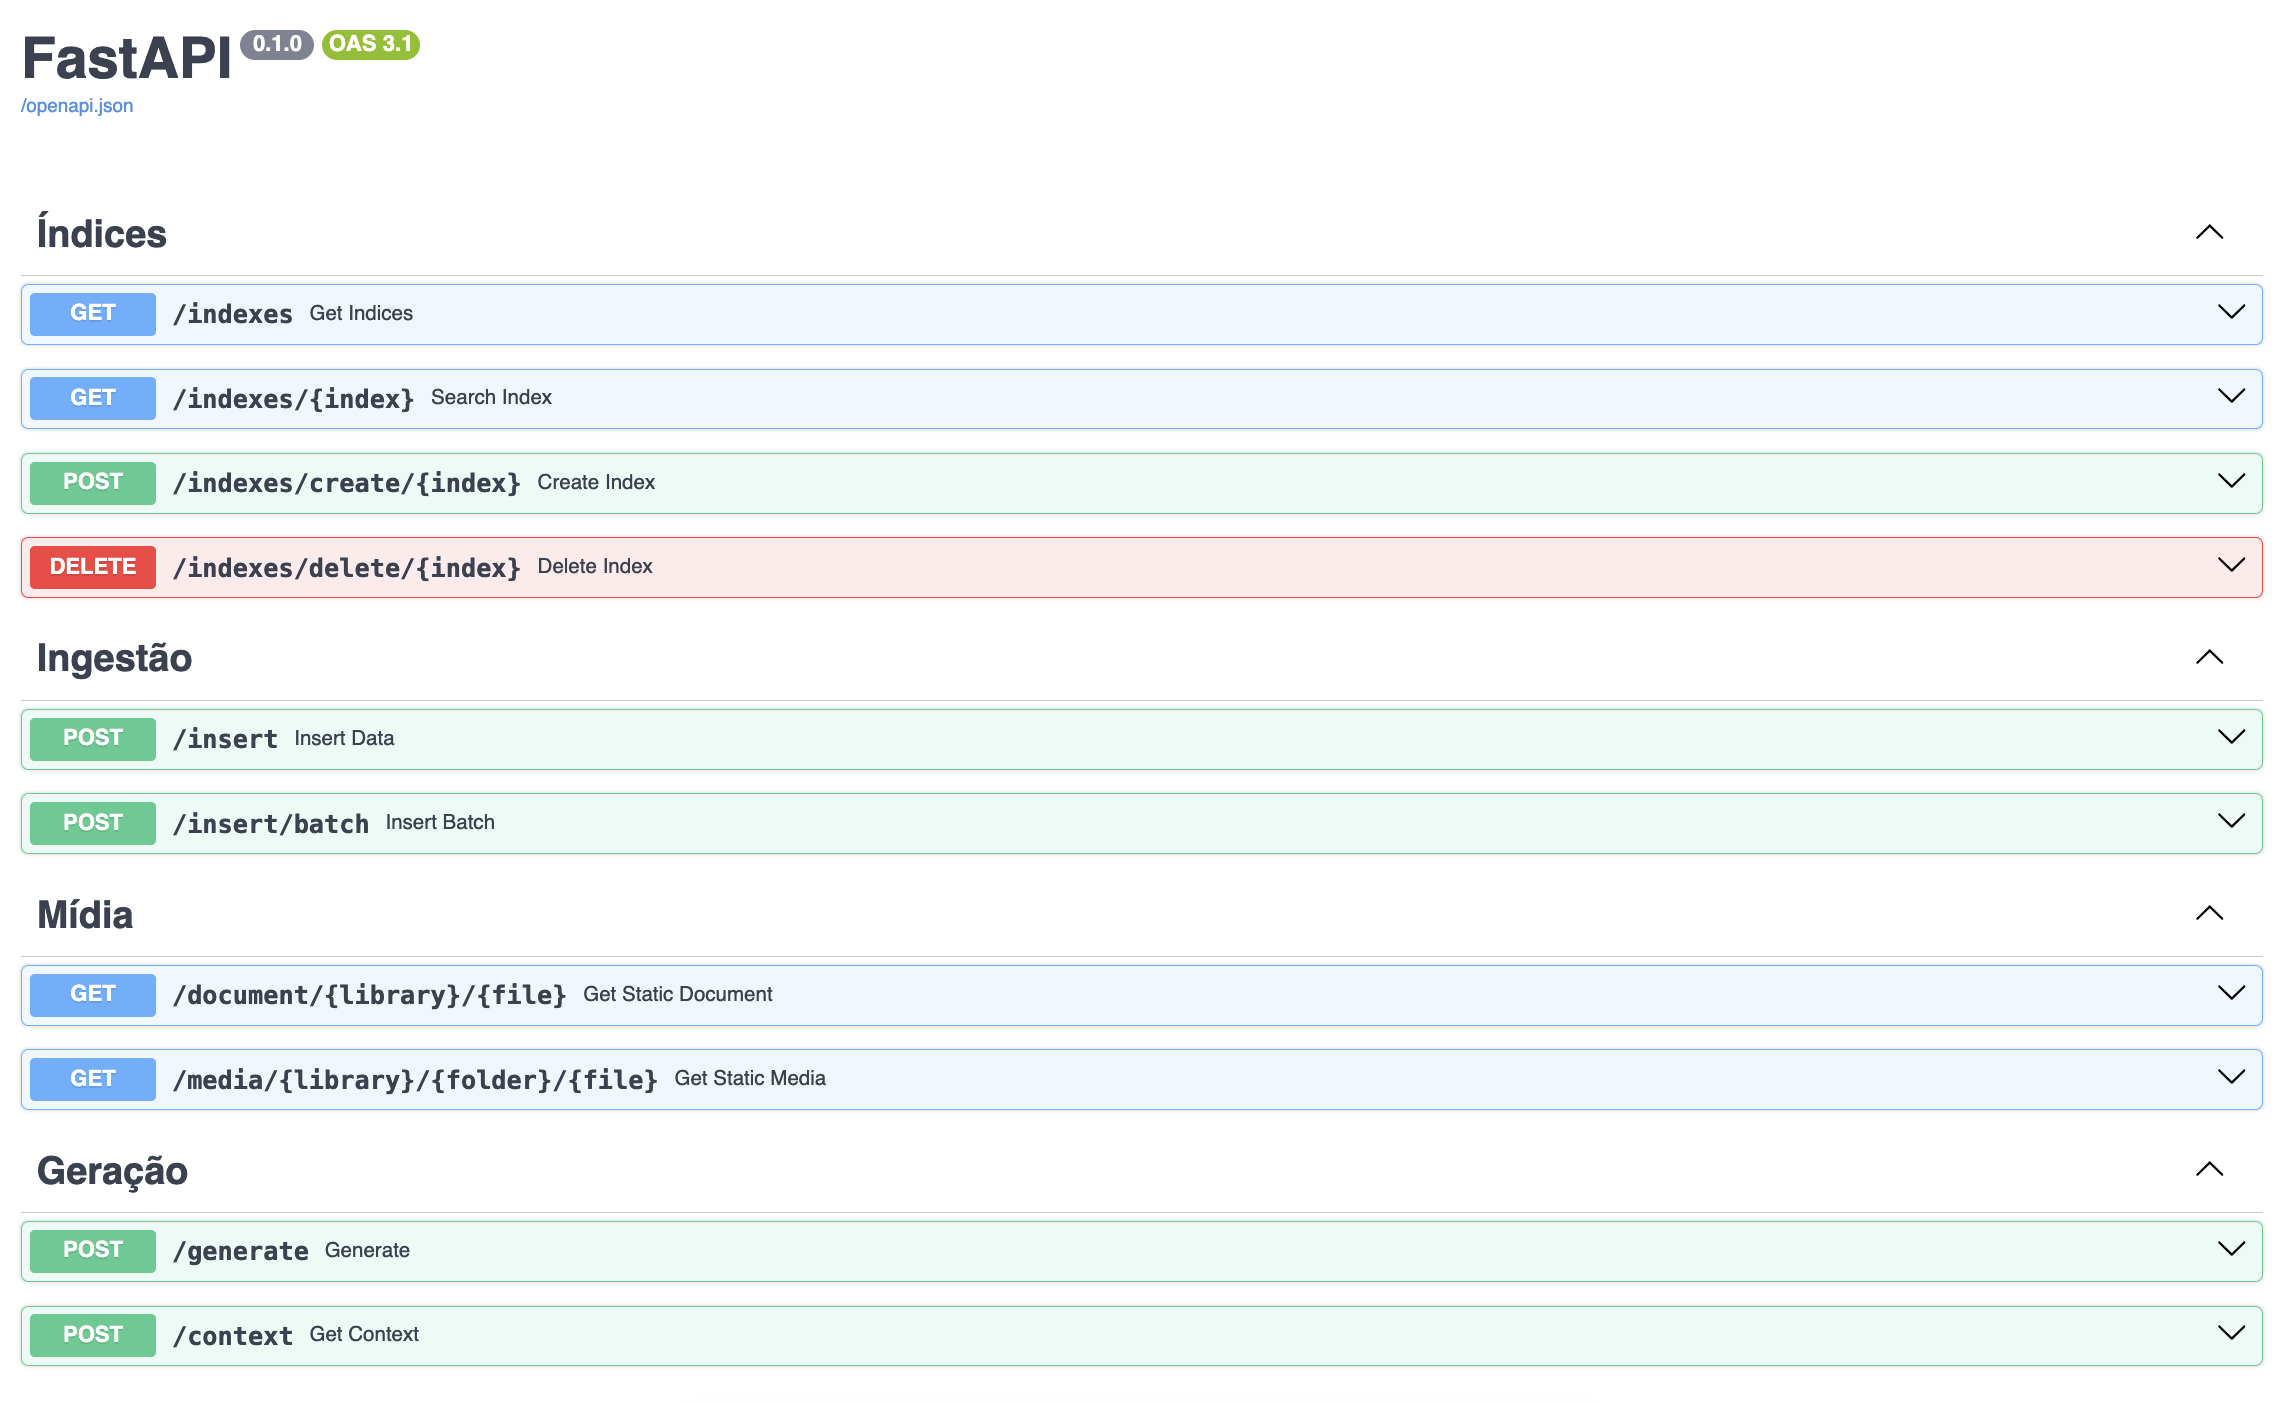
\includegraphics[width=\textwidth,height=0.9\textheight,keepaspectratio]{endpoints.png}
        \centering
        \caption{Visão interativa da documentação, exibindo os \textit{endpoints} disponíveis na API implementada e suas funcionalidades.}
        \centering
        \label{fig:endpoints}
    \end{figure}

    Dentro da visão interativa da documentação proporcionada pela \autoref{fig:endpoints} pode-se descrever cada um dos grupos identificados e seus respectivos \textit{endpoints} da seguinte maneira:

    \begin{enumerate}
        \item \textbf{\textit{Índices}}\\
        Responsáveis por operações relacionadas aos índices da instância do banco vetorial configurado para a aplicação.
        \begin{itemize}
            \item \textbf{\texttt{/indexes}}: Lista todos os índices disponíveis no banco vetorial instanciado.
            \item \textbf{\texttt{/indexes/index}}: Verifica se determinado índice existe ou não, dentro do banco vetorial instanciado.
            \item \textbf{\texttt{/indexes/create/index}}: Efetua a criação de um novo índice para o banco vetorial instanciado.
            \item \textbf{\texttt{/indexes/delete/index}}: Remove um índice, já existente, no banco vetorial instanciado.
        \end{itemize}
        \item \textbf{\textit{Ingestão}}:\\ Responsáveis por todas as operações de ingestão de dados na instância do banco vetorial configurado para a aplicação.
        \begin{itemize}
            \item \textbf{\texttt{/insert}}: Insere um único documento dentro do índice no banco vetorial instanciado
            \item \textbf{\texttt{/insert/batch}}: Insere múltiplos documentos dentro do índice no banco vetorial instanciado, inserindo \textit{batches} ou grupos grandes.
        \end{itemize}
        \item \textbf{\textit{Mídia}}:\\ Responsáveis por operações relacionadas à consulta de mídias, como imagens e documentos processados presentes no orquestrador.
        \begin{itemize}
            \item \textbf{\texttt{document/library/file}}: Retorna um documento que tenha sido previamente processado durante a ingestão (pdf, doc, csv, etc).
            \item \textbf{\texttt{media/library/folder/file}}: Retorna um arquivo de imagem (png ou jpeg).
        \end{itemize}
        \item \textbf{\textit{Geração}}:\\ Responsáveis por operações relacionadas enriquecimento e geração de perguntas e respostas para o usuário.
        \begin{itemize}
            \item \textbf{\texttt{/generate}} \label{sec:generate}: Interpreta uma consulta, em seguida realiza uma busca por contexto no banco vetorial instanciado e usa um LLM para interpretar este contexto e retornar uma resposta humanizada.
            \item \textbf{\texttt{/context}} \label{sec:context}: Busca contexto no banco vetorial instanciado a partir de uma consulta.
        \end{itemize}
    \end{enumerate}

    É importante frisar que todas as operações realizadas no orquestrador envolvendo \textit{embedding} precisam ter o mesmo modelo e dimensões utilizados na configuração e instanciação do serviço de \textit{embedding} adotado durante a etapa de ingestão dos documentos; do contrário, as respostas serão confusas e muitas vezes erradas, correspondendo a alucinações (\textit{hallucinations}).

    Além disso, por se tratar de uma implementação conduzida em um ambiente local, sem \textit{deploy} em servidores externos ou infraestruturas na nuvem, optou-se por não incluir \textit{endpoints} relacionados à segurança da aplicação. Embora a segurança seja um aspecto fundamental em sistemas distribuídos, a natureza controlada do ambiente experimental justifica a exclusão dessa camada adicional, permitindo que o foco permaneça na validação e na funcionalidade do ecossistema em si. Essa decisão não diminui a importância do tema, mas reflete uma abordagem pragmática, alinhada ao escopo definido para este trabalho.

    \subsubsection{\textit{Endpoints} de Geração}

    Como o objetivo principal do ecossistema RAG é gerar uma resposta ao usuário, esta seção irá focar nos dois \textit{endpoints} implementados para o objetivo em questão. O primeiro \textit{endpoint}, resumido no \autoref{sec:generate}, é o responsável pelo fluxo de consultas implementado na interface gráfica. Uma vez enviadas a pergunta, estratégia de busca e biblioteca de documentos na requisição para o orquestrador, o \textit{endpoint} \textit{/generate} identifica a estratégia a ser utilizada, encaminha a pergunta para um serviço responsável pelo \textit{embedding} que, por sua vez, vai formatar a pergunta. Em seguida, é feita uma busca por documentos relevantes dentro da instância do banco vetorial. Essa busca é realizada a partir do segundo \textit{endpoint} implementado, resumido no \autoref{sec:context}, que irá receber a estratégia selecionada e realizar uma busca por documentos relevantes na instância do banco vetorial.

    Com os documentos relevantes encontrados, a partir do \textit{endpoint} \texttt{/context}, o \texttt{/generate} dá continuidade ao seu fluxo e utiliza os documentos relevantes encontrados como contexto para enviar a um serviço de LLM. Neste caso, o \textit{/generate} envia o contexto adquirido, juntamente com a pergunta original feita pelo usuário, ou seja, sem o \textit{embedding}. Após a requisição ao serviço de LLM, o \texttt{/generate} retorna uma resposta humanizada ao usuário.

    \subsubsection{Abstrações de Serviços} \label{sec:abstraction}

    Dentro da API, são utilizados diversos serviços, abrangendo tanto funcionalidades internas, como \textit{logging} e testes, quanto aspectos essenciais para a aplicação, como os serviços de integração com modelos de LLMs e conexão com bancos vetoriais. Para proporcionar maior flexibilidade aos desenvolvedores interessados em estender ou adaptar este trabalho às suas necessidades, além de adicionar uma camada de abstração à aplicação, os serviços de LLM e de conexão com o banco vetorial seguem a mesma abordagem descrita na \autoref{sec:pipeline}, baseada no padrão de fábrica.

    No contexto do orquestrador, o padrão de fábrica é responsável por encapsular a lógica de criação dos serviços de LLM e de conexão com bancos vetoriais (equivalentes ao \textit{product} na \autoref{fig:factory-pattern}), permitindo que os desenvolvedores escolham ou configurem diferentes implementações desses serviços sem modificar a estrutura principal da aplicação. 
    
    Por exemplo, um desenvolvedor pode optar por usar um serviço de LLM específico, como GPT e \textit{LLama}, ou selecionar um banco vetorial diferente, como \textit{Pinecone} \footnote{\citeurl{pinecone}} ou \textit{Elasticsearch} \footnote{\citeurl{elasticsearch}}.
    
    Dessa forma, essa abordagem não apenas reduz o acoplamento entre os componentes, mas também simplifica a adição de novos serviços no futuro. Ao promover uma arquitetura mais organizada e escalável, garante-se que o orquestrador seja acessível a desenvolvedores com diferentes demandas e preferências tecnológicas.

    \subsection{Estratégias de Busca} \label{sec:strategies}

    Como o orquestrador é o principal componente responsável pela comunicação com o banco vetorial instanciado, ela desempenha um papel crucial na implementação de diferentes estratégias de busca para o ecossistema RAG. Existem diversas abordagens utilizadas para a busca de contexto, neste trabalho serão implementadas duas das estratégias descritas no \citetitle{retrieval_strategies}, \citeb{retrieval_strategies} sendo elas a \textit{Vector Store Flat Index} e \textit{Small to Big}. Estratégias de busca adotam maneiras distintas de enriquecer as respostas geradas, o que impacta o resultado final.

    A escolha da estratégia de busca adequada depende diretamente das características da base de dados contida no banco vetorial. Estratégias distintas geram diferentes graus de refinamento e contextualização nas respostas, o que pode ser uma vantagem ou desvantagem, dependendo do objetivo do sistema e da qualidade dos dados armazenados. Por exemplo, bases de dados bem estruturadas e consistentes podem se beneficiar de abordagens mais simples, enquanto bases de dados mais heterogêneas podem exigir estratégias mais sofisticadas, como o uso de modelos ou algoritmos usados para reordenar os documentos recuperados na fase de busca, denominados \textit{rerankers}.

    Para garantir a precisão e a confiabilidade das respostas geradas pelo sistema, é fundamental realizar uma análise de desempenho. Recomenda-se confeccionar uma bateria de perguntas e avaliar as respostas geradas por cada estratégia e para cada biblioteca com que o ecossistema RAG interage.

    A avaliação das respostas geradas irá determinar a qualidade que o ecossistema RAG alcançou em suas respostas. Esta avaliação é essencial para classificar o amadurecimento da solução e deve ser feita através de um ou mais humanos que tenham conhecimento dos dados da biblioteca contida no banco vetorial, ou por \textit{frameworks} projetados para avaliar o desempenho de sistemas RAG, como o \textit{Retrieval Augmented Generation Assessment Suite} (RAGAS), que avalia um sistema RAG em diferentes aspectos.
    
    Esse processo não apenas valida a adequação de cada abordagem, mas também fornece \textit{insights} para ajustes no sistema, garantindo que ele atenda de forma eficaz às necessidades do usuário final.

    No que se segue, serão explicadas as duas estratégias de busca de contexto exploradas neste trabalho.

    \subsubsection{\textit{Vector Store Flat Index}} \label{sec:vector_search}

    O coração do RAG é um índice de busca que organiza o conteúdo em formato vetorizado, permitindo identificar os fragmentos mais relevantes para uma consulta com base em comparações entre os vetores, como discutido no \autoref{sec:recovery}. Essa abordagem, ilustrada na \autoref{fig:vector_strategy}, recebe a consulta do usuário e realiza o \textit{embedding} dela, realizando uma busca vetorial no banco pelos top $k$ \textit{chunks} mais relevantes. 

    \clearpage

    \begin{figure}[ht]
        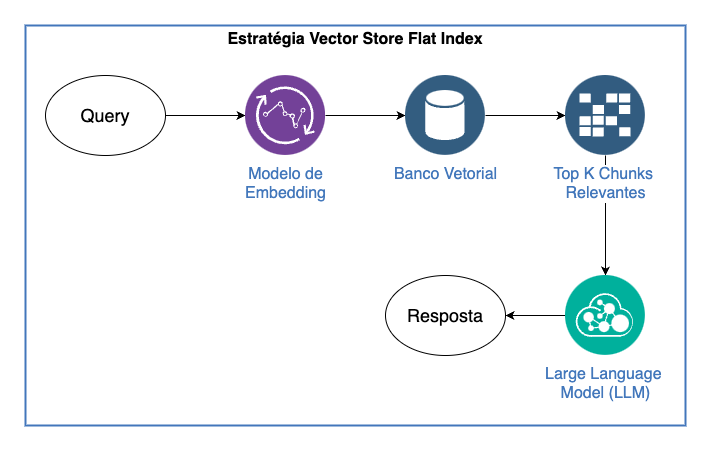
\includegraphics[width=\textwidth,height=0.9\textheight,keepaspectratio]{vector-strategy.png}
        \centering
        \caption{Fluxograma do funcionamento da estratégia \textit{Vector Store Flat Index}.}
        \centering
        \label{fig:vector_strategy}
    \end{figure}

    Em seguida, o contexto dos \textit{chunks} mais relevantes é enviado para um serviço de LLM, que irá receber um \textit{prompt} junto com o contexto e gerar uma resposta humanizada. Além de simples e eficiente, facilita a recuperação de informações relevantes ao priorizar os $k$ fragmentos mais próximos do vetor de consulta.

    \subsubsection{\textit{Small to Big}} \label{sec:small_to_big_search}

    Essa estratégia envolve vincular cada um dos top $k$ \textit{chunks} com seus \textit{chunks} adjacentes, obtendo contextos mais amplos para o LLM. 
    
    Quando os top $k$ \textit{chunks} são identificados, cada um deles é enriquecido, de forma que o \textit{chunk} anterior e o próximo são recuperados a partir de uma chave de sequência instanciada durante a ingestão dos documentos, ou seja, se foi identificado o \textit{chunk} $4$ como relevante, ele será enriquecido com os \textit{chunks} $3$ e $5$ respectivamente. Isso ocorre para cada um dos top $k$ \textit{chunks} relevantes.
    
    Com esta implementação, é possível fornecer um contexto mais amplo para o LLM, como ilustrado na \autoref{fig:small_to_big_strategy}.
    
    \begin{figure}[ht]
        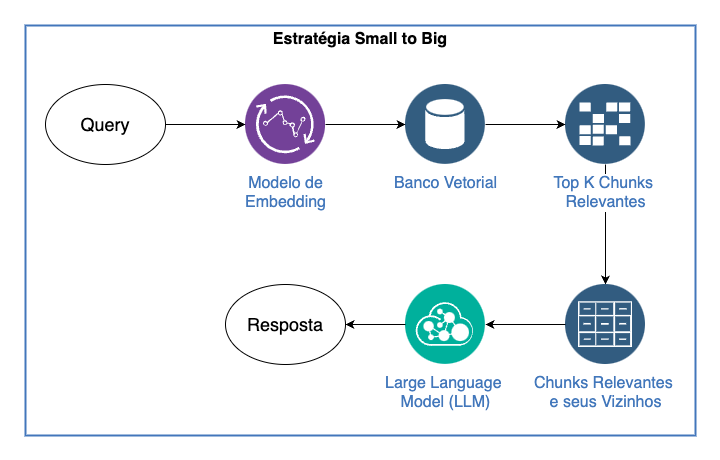
\includegraphics[width=\textwidth,height=0.9\textheight,keepaspectratio]{small-to-big-strategy.png}
        \centering
        \caption{Fluxograma do funcionamento da estratégia \textit{Small to Big}.}
        \centering
        \label{fig:small_to_big_strategy}
    \end{figure}

    

    \subsection{Buscas Vetoriais} \label{sec:vec_search}

    Neste trabalho, foi escolhido o \textit{Elasticsearch}, discutido na \autoref{sec:elasticsearch}, como instância de banco vetorial para a criação de \textit{indexes} e execução de buscas por contexto.

    Nas buscas vetoriais realizadas, são analisados os \textit{embeddings} tanto da consulta quanto aqueles já armazenados no banco de dados, sendo retornado o \textit{nearest neighbor}, ou seja, o resultado mais próximo, segundo uma métrica de similaridade adotada, ao \textit{embedding} correspondente à consulta. Para garantir o retorno do \textit{nearest neighbor}, o \textit{elasticsearch}, faz uso de um algoritmo \textit{Approximate Nearest Neighbor} (ANN), mais especificamente o \textit{Hierarchical Navigable Small World graphs} (HNSW) como evidenciado na publicação da versão $8.0$ do \textit{elasticsearch} \citetitle{hsnw}, \citeb{hsnw}.
    
    O algoritmo ANN encontra um ponto em um conjunto de dados muito próximo ao ponto de consulta fornecido, mas não necessariamente o mais próximo de forma absoluta. Enquanto um algoritmo NN (\textit{Nearest Neighbor}) percorre toda a base de dados, gastando tempo O(n), para encontrar a correspondência perfeita, um algoritmo ANN se contenta com uma correspondência que seja ``próxima o suficiente'' e que possa ser encontrada rapidamente. 
    
    Isso pode parecer uma solução inferior, mas é a chave para realizar buscas rápidas por similaridade. Desta maneira, em vez de consumir uma grande quantidade de tempo e recursos, é possível identificar pontos similares com muito menos esforço, mas que ainda são úteis na maioria dos cenários práticos.
    
    É importante frisar que uma busca vetorial no algoritmo ANN não percorre todo o banco vetorial porque, em conjuntos de dados muito grandes, a busca exaustiva (complexidade O(n)) por cada ponto se torna computacionalmente inviável, demandando tempos de resposta muito altos e consumo excessivo de recursos. 
    
    Para contornar essa limitação, o ANN emprega estruturas de dados especializadas, que permitem navegar apenas pelas regiões do espaço vetorial que têm maior probabilidade de conter os resultados mais relevantes. Isso reduz significativamente o número de comparações necessárias, mantendo a busca eficiente e prática, especialmente em aplicações onde o tempo de resposta é crítico. Essa abordagem é particularmente vantajosa em aplicações em que a escalabilidade e o tempo de resposta são fatores críticos, como em sistemas de recomendação e recuperação de informações.
    

    \subsection{Interface Gráfica de Usuário}
    
    O objetivo principal de uma interface gráfica é proporcionar ao usuário uma experiência intuitiva, eficiente e agradável ao longo de sua interação com os fluxos da aplicação. Uma interface bem projetada não apenas facilita a navegação, mas também reduz a curva de aprendizado e possíveis frustrações. No contexto deste trabalho, como o foco é a simulação de um assistente virtual, a forma mais natural e prática de implementar o ecossistema RAG seria por meio de uma interface de \textit{chat}. Essa escolha se justifica pela familiaridade do público com esse tipo de interação, especialmente em cenários de assistência automatizada, permitindo que o usuário obtenha respostas às suas dúvidas e perguntas de maneira direta e acessível.

    Para viabilizar essa proposta, foi utilizada a biblioteca \textit{streamlit}, apresentada na \autoref{sec:streamlit}, que possibilita a criação rápida e interativa de interfaces \textit{web}. A partir dessa tecnologia, foi desenvolvida uma interface de \textit{chat} que simula o comportamento de um assistente virtual, apresentada na \autoref{fig:chat_interface}. A estrutura da interface foi planejada para maximizar a usabilidade e a organização da interação.
    
    \begin{figure}[ht]
        
\includegraphics[width=\textwidth,height=0.9\textheight,keepaspectratio]{chat-interface.png}
        \centering
        \caption{Interface de chat implementada com uso da biblioteca \textit{streamlit}.}
        \centering
        \label{fig:chat_interface}
    \end{figure}

    Na \autoref{fig:chat_interface}, na barra lateral à esquerda, encontram-se dois filtros que fornecem ao usuário controle sobre dois parâmetros do sistema: 
    
    \begin{enumerate}
        \item \textbf{Seletor de bibliotecas}: embora neste trabalho o escopo de bibliotecas esteja limitado a uma única opção, a escalabilidade do projeto está presente. Esta opção permite que um desenvolvedor possa realizar a ingestão de múltiplas bibliotecas;
        \item \textbf{Seletor de estratégia de busca}: permite que o usuário escolha determinada estratégia de busca para obter respostas mais precisas dependendo dos dados presentes na biblioteca, como discutido na \autoref{sec:strategies}.
    \end{enumerate}
    
    Esses seletores possibilitam a personalização da experiência do usuário e um ajuste em tempo real do contexto que será buscado de acordo com as possíveis configurações.

    Ainda na \autoref{fig:chat_interface}, no plano central da interface, está localizado o \texit{chat} propriamente dito, que exibe as mensagens trocadas entre o usuário e o assistente virtual. Essa área principal é responsável por gerenciar as interações do usuário com o orquestrador subjacente, fornecendo respostas e implementando o comportamento de um sistema de perguntas e respostas. O design foi cuidadosamente planejado para que a comunicação seja clara, eficiente e visualmente organizada, reforçando o objetivo de criar uma experiência fluida e satisfatória ao usuário.

    \clearpage

    \section{Avaliação Experimental} \label{sec:experiment}

    Como dito anteriormente na \autoref{sec:objectives}, um dos objetivos específicos deste trabalho é executar uma validação sobre a solução gerada, de maneira que o resultado seja relevante. Ou seja, é necessário avaliar a eficácia e viabilidade do ecossistema a fim de responder se ele é capaz ou não de sanar dúvidas ou responder perguntas acerca de um determinado conjunto de documentos, de maneira satisfatória. 

    Assim, para a realização da avaliação, como discutido na \autoref{sec:data}, foi feita a inserção de um conjunto de dados menor, totalizando 22 documentos do tipo \textit{PDF} com TCCs de diversos alunos do curso. A inserção dos dados demorou cerca de 44 minutos e utilizou-se o modelo \textit{\textbf{intfloat/multilingual-e5-base}} para os \textit{embeddings}. Para o funcionamento do pipeline de ingestão, foram utilizados os parâmetros do \autoref{lst:ingestion_params}, baseando-se no \autoref{lst:env_params}

    \begin{lstlisting}[caption={Objeto com os parâmetros da configuração de ambiente do pipeline de ingestão.}, label={lst:ingestion_params}]
        {
            "EXTRACTION_DATABASE": "bsi",
            "DATA_PATH": "data",
            "MEDIA_PATH": "media",
            "RESULTS_PATH": "results",
            "EMBEDDING_MODEL": "intfloat/multilingual-e5-base",
            "EMBEDDING_DIMENSIONS": 384,
            "CHUNK_MAX_LEN": 1024,
            "INGESTION_BATCH": 500,
        }
    \end{lstlisting}

    \subsection{Definição do Experimento}
    
    Assim, nesta avaliação, serão necessários um \textit{prompt} para o assistente, perguntas e definição de estratégia de busca para se obterem os resultados necessários para preencher o \textit{template} proposto na \autoref{tab:template_results}. Como foi explicado na \autoref{sec:gui}, mais especificamente na etapa 4 da \autoref{fig:gui_scheme}, é necessário encaminhar um \textit{prompt} que será utilizado durante as requisições ao serviço de LLM no enriquecimento das respostas. Para esta avaliação, o \textit{prompt} é:

    \begin{quote}
        
    \textit{Você é o assistente prestativo da UNIRIO, cujo trabalho é auxiliar estudantes e pesquisadores a esclarecer dúvidas sobre os trabalhos de conclusão de curso (TCCs).
    Seu trabalho é responder as perguntas de forma clara, utilizando somente os dados disponíveis dentro das tags de <context> e <history> fornecidas.
    Sempre que for solicitado uma lista com ``todos os trabalhos'' ou ``todas as citações'', deixe claro que você irá retornar uma partição da biblioteca.}
    
    \textit{Antes de responder, você precisa identificar e analisar as seguintes tags:
        1. Tag <query> que identifica o começo de uma pergunta (</query> identifica o fim da pergunta).
        2. Tag <context> que comporta as informações achadas, sobre a pergunta, dentro do banco de dados de TCCs da UNIRIO (</context> identifica o fim do contexto).
        3. Tag <history> que identifica o histórico da conversa, no formato "[role]: [mensagem]" (</history> identifica o fim do histórico).}
    
    \textit{Acima de tudo, além de ser um assistente prestativo, você deve seguir única e exclusivamente as regras a seguir. Caso contrário, será punido e desligado.
        1. Quando não tiver certeza da resposta diga sinceramente que não possui informações suficientes sobre esse tema.
        2. Toda resposta deve estar em formato markdown, para ser usado no framework streamlit. As respostas não devem possuir cabeçalhos.
        3. Dentro de toda resposta, você deve utilizar somente os dados dentro da tag <context> e <history>}
        
    \end{quote}
    
    Para isso, com o objetivo de avaliar o ecossistema implementado, foram preparadas três perguntas referentes ao conjunto de dados da biblioteca escolhida na \autoref{sec:data}. Estas perguntas têm o objetivo de buscar informações gerais, específicas e abrangentes da biblioteca, sendo elas:

    \begin{enumerate}
        \item Gostaria de saber quais trabalhos abordam o tema ``acessibilidade''.
        \item Existe algum trabalho que aborde a implementação de uma API?
        \item Liste todos os trabalhos que abordem o tema ``inteligência artificial''.
    \end{enumerate}

    Cada uma dessas perguntas será realizada para cada estratégia de busca implementada, sendo elas representadas pelas seguintes chaves:
    
    \begin{itemize}
        \item \textbf{\textit{vector}}: estratégia \textit{Vector Store Flat Index} discutida na \autoref{sec:vector_search}.
        \item \textbf{\textit{small to big}}: estratégia \textit{Small to Big} discutida na \autoref{sec:small_to_big_search};
    \end{itemize}
    
    No final das requisições haverá uma tabela, contendo o número da pergunta, a estratégia de busca e um valor indicando se a resposta foi satisfatória, insatisfatória ou uma alucinação (a partir de uma classificação humana). Como ilustrado na \autoref{tab:template_results} a seguir:

    \begin{center}
        \begin{table}[h!]
        \centering
        \renewcommand{\arraystretch}{1.5} % Ajusta a altura das linhas
        \setlength{\tabcolsep}{8pt} % Ajusta a largura entre colunas
        \begin{tabular}{|c|c|l|}
        \hline
        \textbf{Pergunta} & \textbf{Estratégia de Busca} & \textbf{Resposta} \\ \hline
         1                & \textit{vector}              & Satisfatória      \\ \hline
         2                & \textit{small to big}        & Alucinação        \\ \hline
         3                & \textit{vector}              & Insatisfatória    \\ \hline
        \end{tabular}
        \caption{Exemplo de tabela para os resultados do experimento.}
        \label{tab:template_results}
        \end{table}
    \end{center}

    Uma resposta é considerada \textbf{satisfatória}, por um avaliador humano, quando o assistente fornecer uma resposta contextualizada, acompanhada dos documentos que contenham o conteúdo pertinente à pergunta realizada. Caso o assistente forneça apenas a referência aos documentos, sem contextualizar a resposta, esta será considerada \textbf{insatisfatória}, por um avaliador humano, pois não atendeu à expectativa de uma ``resposta humanizada''.

    Quando o assistente não entregar nem uma resposta contextualizada nem referenciar documentos relevantes ao contexto da pergunta, a resposta será classificada como uma \textbf{alucinação}, pois o conteúdo gerado ou referenciado não tem relação com a consulta feita. Essa classificação é essencial para analisar a relevância e a contextualização das respostas geradas pelo modelo, especialmente em cenários que demandem alta qualidade informacional e precisão contextual.
    
    \subsection{Resultados} \label{sec:results}

    Neste trabalho, a qualidade das respostas do assistente é avaliada com base nos critérios de relevância e contextualização, onde um documento só é relevante se abordar o tema de uma consulta e a contextualização é considerada satisfatória quando o assistente discorre sobre os documentos encontrados, e insatisfatória quando o assistente não souber responder ou não encontrar material suficiente para formular uma resposta humanizada. Após a realização do experimento e a aplicação desses critérios, os resultados obtidos são apresentados na \autoref{tab:results}.
    
    \begin{center}
        \begin{table}[h!]
        \centering
        \renewcommand{\arraystretch}{1.5} % Ajusta a altura das linhas
        \setlength{\tabcolsep}{8pt} % Ajusta a largura entre colunas
        \begin{tabular}{|c|c|l|}
        \hline
        \textbf{Pergunta} & \textbf{Estratégia de Busca} & \textbf{Resposta} \\ \hline
         1                & \textit{vector}        & Satisfatória   \\ \hline
         2                & \textit{vector}        & Satisfatória   \\ \hline
         3                & \textit{vector}        & Insatisfatória \\ \hline
         1                & \textit{small to big}  & Satisfatória.  \\ \hline
         2                & \textit{small to big}  & Satisfatória   \\ \hline
         3                & \textit{small to big}  & Insatisfatória \\ \hline
        \end{tabular}
        \caption{Tabela com os resultados do experimento modelado.}
        \label{tab:results}
        \end{table}
    \end{center}

    % \clearpage
    
    \begin{figure}[ht]
        \includegraphics[width=\textwidth,height=0.9\textheight,keepaspectratio]{vector-question-1.png}
        \centering
        \caption{Pergunta 1 sendo feita através da estratégia de busca \textit{Vector Store Flat index}.}
        \centering
        \label{fig:satisfactory-question}
    \end{figure}
    
    Na \autoref{fig:satisfactory-question}, tem-se um exemplo de resposta satisfatória durante a execução da primeira pergunta utilizando a estratégia de \textit{Vector Store Flat Index}.
    
    Nesta execução, perguntando sobre TCCs que abordam o tema da acessibilidade, observa-se que o assistente trouxe uma resposta com um único documento, evidenciando as três páginas do documento onde foi identificada uma maior similaridade com a pergunta. Além disso, o assistente retorna o título do trabalho, seguido de um alerta ``Essa é apenas uma parte da biblioteca. Se você deseja mais informações, entre em contato com o departamento de TCCs da UNIRIO.'', embora o departamento de TCCs da UNIRIO não exista, o assistente deixa evidente que pode haver mais trabalhos que abordem o tema, como discutido na \autoref{sec:vec_search}.

    \begin{figure}[ht]
        \includegraphics[width=\textwidth,height=0.9\textheight,keepaspectratio]{vector-question-2.png}
        \centering
        \caption{Pergunta 2 sendo feita através da estratégia de busca \textit{Vector Store Flat index}.}
        \centering
        \label{fig:satisfactory-question-B}
    \end{figure}

    Outro exemplo de resposta satisfatória pode ser observado na \autoref{fig:satisfactory-question-B}, em que foi perguntado sobre TCCs que abordem a implementação de uma API, de forma que o assistente retornou dois documentos. O primeiro documento se trata do documento principal, do qual o assistente expôs as seções 4 e 5 em sua resposta. Entretanto, no segundo documento, há somente duas menções à palavra API em entrevistas feitas pela autora e, portanto, não entraram para o contexto da resposta humanizada.

    \clearpage
    
    \begin{figure}[ht]
        \includegraphics[width=\textwidth,height=0.9\textheight,keepaspectratio]{vector-question-3.png}
        \centering
        \caption{Pergunta 3 sendo feita através da estratégia de busca \textit{Vector Store Flat index}.}
        \centering
        \label{fig:insatisfactory-question}
    \end{figure}

    Na execução da terceira pergunta, ilustrada na \autoref{fig:insatisfactory-question}, foi solicitada a listagem de trabalhos que abordem inteligência artificial, em que é possível observar que o assistente fornece uma resposta insatisfatória. E como discutido na \autoref{sec:vec_search}, no contexto de busca vetorial abordado no ecossistema RAG não são executadas buscas exaustivas pelo banco. Assim, em consultas onde um usuário busca por ``todas as menções'' ou ``todos os documentos'', o ecossistema RAG abordado neste trabalho não é a melhor estrutura para sanar esse tipo de problema. 
    
    Nestes cenários, é necessária uma busca exaustiva pelo banco ou uma estrutura auxiliar que possa ser consumida pelo componente orquestrador, onde seja feita a busca exaustiva ou o consumo de um mapeamento prévio dos documentos presentes no banco vetorial. Ainda assim, a resposta gerada não configura uma alucinação pois, de fato, não há trabalhos que abordem o tema inteligência artificial. 
    
    O assistente alega que não encontrou nenhuma informação sobre trabalhos relacionados ao tema ``inteligência artificial'' e expõe três documentos que não abordam o tema, mas que, nas páginas apontadas, contêm palavras como ``inteligibilidade'', a qual possui uma representação de \textit{embedding} próxima às palavras ``inteligência artificial'', sendo capturada pela similaridade vetorial.

    \clearpage
    
    \begin{figure}[ht]
        \includegraphics[width=\textwidth,height=0.9\textheight,keepaspectratio]{stb-question-1.png}
        \centering
        \caption{Pergunta 1 sendo feita através da estratégia de busca \textit{Small to Big}.}
        \centering
        \label{fig:satisfactory-question-C}
    \end{figure}
    
    Ao se executarem as perguntas para a estratégia de busca \textit{Small to Big}, observa-se que as respostas são muito similares mesmo com a troca de estratégia. Contudo, percebe-se que essa estratégia é capaz de referenciar mais documentos que a estratégia \textit{Vector Store Flat Index}, mesmo que os demais documentos não sejam tão relevantes quanto o primeiro, como visto na \autoref{fig:satisfactory-question-C}, em que somente o primeiro documento se relaciona com a consulta feita. Também é possível observar que ambas as estratégias obtiveram a mesma referência como primeiro documento, inclusive considerando as páginas referenciadas, conforme as \autoref{fig:satisfactory-question} e \autoref{fig:satisfactory-question-C} embora a estratégia \textit{Small to Big} também tenha retornado outros documentos, devido ao seu comportamento, discutido na \autoref{sec:small_to_big_search}.

    A partir da \autoref{tab:results}, observa-se que, independente da estratégia escolhida para a biblioteca de TCCs abordada, a qualidade das respostas é a mesma. Os únicos pontos de atenção correspondem à quantidade de documentos referenciados nas estratégias, que possuem implementações distintas. Além disso, também é necessário ter atenção às consultas que peçam para ``listar todos...'' ou ``citar todas...'', pois no contexto de busca vetorial abordado na \autoref{sec:vec_search}, acaba sendo infactível, já que não é realizada uma busca exaustiva no banco vetorial ao buscar por um contexto.

    \clearpage
    
    \section{Conclusão}
    
    \subsection{Considerações Finais}

    A era digital, impulsionada pela expansão da Internet das Coisas (IoT), colocou os seres humanos no centro de um turbilhão de informações, em que cada indivíduo, por meio de dispositivos conectados, se tornou não apenas consumidor, mas também criador de dados em larga escala. \textit{Smartphones}, dispositivos inteligentes e plataformas on-line produzem continuamente um rastro digital, transformando nossas atividades diárias em peças de um imenso quebra-cabeça global. Esse cenário destaca um paradoxo intrigante, pois enquanto as tecnologias facilitam a comunicação e o acesso ao conhecimento, o volume cada vez maior de dados gerados ultrapassa a capacidade humana de absorção. A era do ``excesso de dados'' desafia as pessoas a encontrarem maneiras mais inteligentes de filtrar, interpretar e aproveitar essa riqueza de informações sem se perderem em sua imensidão.

    No contexto do cenário atual, marcado pelo crescente volume de dados gerados diariamente e pela presença de vastas bibliotecas digitais, a busca por informações tornou-se uma tarefa cada vez mais desafiadora, exigindo soluções que combinem eficiência e acessibilidade.

    Diante do desafio de lidar com o excesso de informações, a tecnologia RAG surge como uma solução para transformar grandes bibliotecas de dados em fontes acessíveis e inteligentes. Combinando recuperação de informações relevantes e geração de texto baseada em IA, o RAG permite que o usuário obtenha respostas precisas e contextualizadas de maneira rápida e intuitiva. Localizando informações relevantes em vastos repositórios, processa o conteúdo e apresenta respostas claras, eliminando a necessidade de se navegar por volumes massivos de dados.
    
    Com o objetivo de implementar uma solução baseada em RAG que seja agnóstica aos modelos de LLM e \textit{embedding}, dando liberdade para utilizar qualquer modelo disponível ao desenvolvedor, este trabalho apresenta um ecossistema RAG projetado para melhorar essa interação, oferecendo um sistema capaz de analisar, processar e interagir com qualquer biblioteca de documentos. A proposta contempla um ambiente de desenvolvimento modular e escalonável, permitindo que desenvolvedores integrem novos recursos e aprimorem funcionalidades com facilidade. Além disso, também contempla uma interface gráfica intuitiva desenhada para atender usuários comuns, garantindo que mesmo aqueles sem conhecimentos técnicos possam acessar informações de maneira rápida, precisa e amigável, transformando dados dispersos em \textit{insights} práticos e acessíveis. 

    Em alinhamento com o objetivo de implementar o ecossistema RAG, este trabalho detalha de forma abrangente a modelagem da solução desenvolvida, apresentando as tecnologias empregadas e explicando minuciosamente a arquitetura do sistema, incluindo cada componente implementado e seu papel na integração do ecossistema. Portanto, uma das contribuições deste trabalho é justamente a produção de um documento que instrui a implementação de um ecossistema RAG e tem potencial para introduzir alunos de graduação, entre os quais os do BSI, ao conceito de RAG.
    
    Além disso, para verificar a viabilidade prática da solução, foi realizado um experimento utilizando como base a biblioteca de TCCs do BSI da UNIRIO, considerando o ano de 2023. Neste estudo piloto, foram selecionadas três perguntas que exigissem buscas distintas do ecossistema, paralelo a duas estratégias de busca distintas, em relação a duas estratégias de busca distintas, a \textit{Vector Store Flat Index} e \textit{Small to Big}.
    
    Os resultados obtidos nesse estudo piloto evidenciam o potencial do ecossistema, dado que não houve alucinações dentro das respostas obtidas, demonstrando sua capacidade de processar e organizar informações de maneira eficiente e intuitiva, por meio de uma interface de \textit{chat}, posicionando-se como uma potencial alternativa para contextos reais e em bibliotecas maiores que a abordada.

    \subsection{Limitações}

    O componente de \textit{pipeline} de ingestão, responsável pela análise e processamento das bibliotecas, apresenta características particulares no que diz respeito à capacidade de processamento. O desenvolvedor encarregado de executar esse \textit{pipeline} precisa garantir que a máquina utilizada tenha desempenho suficiente para lidar com bibliotecas de documentos de maior porte. Como o processamento, por padrão, é realizado pela CPU (\textit{Central Processing Unit}), torna-se fundamental avaliar previamente o tamanho da biblioteca e, se necessário, adotar estratégias personalizadas para dividir o processamento em etapas menores, tal como aquela descrita na \autoref{sec:data}. Além disso, é recomendável considerar o uso de uma máquina mais robusta, equipada com uma GPU (\textit{Graphic Processing Unit}), que pode acelerar significativamente o processamento, especialmente em cenários que demandam grande capacidade computacional. Essa abordagem assegura um fluxo mais eficiente e evita possíveis gargalos durante a ingestão e processamento dos dados.

    Alguns LLMS e modelos de \textit{embedding} são soluções privadas, de modo que o acesso a esses recursos exige que o desenvolvedor tenha uma conta ou assinatura ativa junto ao provedor do serviço. Esse processo inclui a geração de uma chave exclusiva, geralmente denominada API \textit{key}, que funciona como uma credencial de acesso. Essa chave autoriza a utilização do LLM ou modelo de \textit{embedding} dentro dos limites estabelecidos pelo provedor, permitindo sua integração e uso eficiente no ecossistema proposto neste trabalho. Essa abordagem garante segurança no acesso, além de possibilitar o rastreamento e o controle do uso dos serviços, essenciais para a implementação de soluções robustas e escaláveis.

    \subsection{Trabalhos Futuros}
    
    Para trabalhos futuros, pretende-se realizar experimentos focados na implementação e avaliação de estratégias de busca adaptativas, capazes de analisar e selecionar automaticamente a abordagem mais eficaz para cada biblioteca de documentos. Isso permitiria a integração do ecossistema RAG proposto de maneira que o usuário não precisasse se preocupar em escolher uma estratégia específica de busca, pois o sistema seria inteligente o suficiente para vincular cada biblioteca à estratégia de busca mais adequada, com base em suas características e necessidades específicas.

    Além da estratégia de busca vinculada à biblioteca, um trabalho que analise determinada biblioteca de documentos e encontre a melhor forma de fazer a divisão de documentos em \textit{chunks} de acordo com a natureza dos documentos presentes na biblioteca pode gerar respostas ainda melhores.

    Outro interesse seria realizar avaliações do ecossistema proposto neste trabalho por especialistas no domínio abordado. Ou seja, se tratando dos TCCs do BSI da UNIRIO, seriam reunidos professores do BSI e montada uma lista de perguntas para serem executadas para o assistente. A partir da resposta dessas perguntas, seria feita uma avaliação humana em conjunto com os professores especialistas no domínio. A partir dessa avaliação, o assistente pode ser classificado como satisfatório ou não.

    Embora os resultados obtidos neste trabalho tenham sido satisfatórios para a biblioteca analisada, em cenários com múltiplas bibliotecas ou bibliotecas compostas por documentos de diferentes temáticas e estruturas, a abordagem se torna mais complexa. Nesse contexto, seria vantajoso contar com uma coleção diversificada de estratégias de busca, implementadas na API, permitindo respostas mais ricas e contextualmente relevantes. A escolha da estratégia ideal para cada biblioteca seria automatizada, utilizando um sistema de pontuação (\textit{score}) atribuído durante a análise da biblioteca no \textit{pipeline} de ingestão. Esse \textit{score} consideraria aspectos como o tipo de conteúdo, a complexidade do tema e a natureza dos dados presentes, permitindo ao ecossistema ajustar suas estratégias de forma dinâmica e eficiente, oferecendo uma experiência mais personalizada e eficaz para o usuário final.

    \clearpage

    \section{Referências}

    \nocite{*}

    % flush section font left
    \sectionfont{\raggedright}
    \printbibliography
    
\end{document}
